\documentclass[11pt,letterpaper]{article}
%\setlength{\textwidth}{14cm}
\usepackage[margin=3cm]{geometry}
\usepackage[utf8]{inputenc}
\usepackage{colortbl}
\usepackage[spanish]{babel}
\usepackage{amsmath}
\usepackage{etoolbox}
\usepackage{amsfonts}
\usepackage{amssymb}
\usepackage{graphicx}
\usepackage{pdflscape}
\usepackage{afterpage}
\usepackage{cite}
\usepackage{footnote}
\usepackage{capt-of}
\usepackage{float}
%\usepackage{times}
%\usepackage{dsfont}
\usepackage{hyperref}
\hypersetup{
    bookmarks=false,         % show bookmarks bar
    unicode=false,          % non-Latin characters in Acrobat’s bookmarks
    pdftoolbar=true,        % show Acrobat’s toolbar?
    pdfmenubar=true,        % show Acrobat’s menu?
    pdffitwindow=false,     % window fit to page when opened
    pdfstartview={FitH},    % fits the width of the page to the window
    pdftitle={Anteproyecto: Trabajo de grado},    % title
    pdfauthor={Carlos Alfredo Cuartas Vélez},     % author
    pdfsubject={Anteproyecto},   % subject of the document
    %pdfcreator={Creator},   % creator of the document
    %pdfproducer={Producer}, % producer of the document
    %pdfkeywords={Phase Diversity} {Fase} {Aberración} {Vórtice Óptico}, % list of keywords
    pdfnewwindow=true,      % links in new window
    colorlinks=True,       % false: boxed links; true: colored links
    linkcolor=red,          % color of internal links (change box color with linkbordercolor)
    citecolor=blue,        % color of links to bibliography
    filecolor=magenta,      % color of file links
    urlcolor=cyan           % color of external links
}

%\setlength{\parindent}{0pt}

\newcommand{\etal}{\emph{et al.} }
\newcommand{\invivo}{\emph{in-vivo} }
\newcommand{\exvivo}{\emph{ex-vivo} }

\begin{document}
	
	\renewcommand{\listfigurename}{Lista de Figuras}
	\renewcommand{\listtablename}{Lista de Tablas}
	\renewcommand{\contentsname}{Contenido}
	\renewcommand{\tablename}{Tabla} 
	\renewcommand{\bibname}{Referencias}
	
	\author{Carlos Alfredo Cuartas Vélez}
\title{Formación y restauración de imagen en tomografía óptica de coherencia mediante posprocesamiento}

\newcommand\portada{
	\begin{titlepage}
		\begin{center}
			\vfill
			{\large  ANTEPROYECTO: TRABAJO DE GRADO}
			\vfill
			\vfill
			{\large  Carlos Alfredo Cuartas Vélez\\
			ccuarta1@eafit.edu.co \par}
			\vfill
			
			{\normalsize  Escuela de Ciencias \par}
			{\normalsize  Departamento de Ciencias Físicas \par}
			{\normalsize  Maestría en Física Aplicada \par}
			{\normalsize  Universidad EAFIT \par}
			{\normalsize  2016\par}
		\end{center}
	\end{titlepage}
}

\newcommand\contraportada{
	\begin{titlepage}
		\begin{center}
			{\large  FORMACIÓN Y RESTAURACIÓN DE IMAGEN EN TOMOGRAFÍA ÓPTICA DE COHERENCIA MEDIANTE POSPROCESAMIENTO}
			\vfill
			{\large  CARLOS ALFREDO CUARTAS VÉLEZ \par} %Cód 201320001163}
			%{\normalsize ccuarta1@eafit.edu.co}
			\vfill
			{\large  ANTEPROYECTO: TRABAJO DE GRADO}
			\vfill
			{\large Director \par} 
            {\large Ph.D. RENÉ RESTREPO GÓMEZ \par}
            {\normalsize Universidad EAFIT \par}
            \vfil
            \vspace{18pt}
            {\large  Co-director \par}
            {\large  Ph.D. NÉSTOR URIBE PATARROYO \par}                        
            {\normalsize Wellman Center for Photomedicine, Harvard Medical School and Massachusetts General Hospital \par}
			\vfill
			
			{\normalsize  ESCUELA DE CIENCIAS \par}
			{\normalsize  DEPARTAMENTO DE CIENCIAS FÍSICAS \par}
			{\normalsize  MAESTRÍA EN FÍSICA APLICADA \par}
			{\normalsize  UNIVERSIDAD EAFIT \par}
			{\normalsize  2016\par}
		\end{center}
\end{titlepage}
}

\portada 
\thispagestyle{empty}

\newpage\null\thispagestyle{empty}\newpage

\contraportada
\thispagestyle{empty}
\newpage\null\thispagestyle{empty}\newpage

\thispagestyle{empty}
\newpage

	\tableofcontents
\newpage
	\section{Introducción}

%La tomografía óptica de coherencia (OCT) es una técnica que permite producir imágenes con alta resolución de la sección transversal y volumétricas de microestructuras internas en tejidos biológicos mediante la medición del ``eco'' producido por la retroreflexión de luz en el tejido \cite{Huang}. El ``eco'' se produce cuando un haz de luz llega hasta el tejido y luego es dispersado, de forma que la información recolectada por la OCT es únicamente aquella porción de luz que es retrodispersada o retroreflejada hacia el sistema óptico. Esta característica permite que la OCT pueda presentar imágenes \emph{in situ} y en tiempo real de patologías presentes en tejidos. Desde su aparición, la OCT ha sido una herramienta útil en el diagnóstico médico, ya que realiza ``biopsias ópticas'' sin la necesidad de remover o procesar parte del tejido \cite{Brezinski1996}, además, es capaz de producir imágenes tridimensionales no invasivas de estructuras internas, tales como la mácula \cite{Hee1995_4}, el tracto gastrointestinal \cite{Tearney1997}, las arterias coronarias \cite{Tearney1996_2}, entre otros.

La tomografía óptica de coherencia (OCT) es una técnica que permite producir imágenes con alta resolución de la sección transversal y/o volumétricas de microestructuras internas en tejidos biológicos, mediante la medición del ``eco'' producido por la retroreflexión de luz en el tejido \cite{Huang1991}. El ``eco'' se produce cuando un haz de luz llega hasta el tejido y luego es dispersado, de forma que la información recolectada por la OCT es únicamente aquella porción de luz retrodispersada o retroreflejada hacia el sistema óptico. Esta característica permite que la OCT pueda presentar imágenes \emph{in-situ} y en tiempo real de patologías presentes en los tejidos, lo que la ha convertido en una herramienta útil en el diagnóstico médico, debido a que realiza ``biopsias ópticas'' sin la necesidad de remover o procesar parte del tejido \cite{Brezinski1996}. La OCT puede producir imágenes tridimensionales \emph{no invasivas} de estructuras internas, tales como la mácula \cite{Hee1995_4}, el tracto gastrointestinal \cite{Tearney1997}, las arterias coronarias \cite{Tearney1996_2}, entre otros.


%% OCT captura imágenes volumétricas mediante la medida de la magnitud y tiempo que tarda una onda de luz en ser retrodispersada por el tejido \cite{Huang}, en este sentido, OCT es análogo al ultrasonido, con la diferencia de que posee una mayor resolución axial, pero una menor profundidad de penetración. La luz retrodispersada se mide empleando interferometría de baja coherencia, también conocida como interferometría con luz blanca, en donde se captura el patrón de interferencia que es producido por un haz de referencia y un haz objeto empleando una fuente con un ancho espectral grande \cite{Tomlins,Fercher}. El haz de referencia es aquel que proviene de la fuente y viaja de manera directa hasta el detector, mientras que el haz objeto es aquella porción de la luz que luego de ser retrodispersada por la muestra, viaja en la dirección del detector. Como la fuente tiene un ancho espectral que abarca varias longitudes de onda la interferencia entre el haz objeto y referencia solo se produce en una región donde la diferencia de camino entre ambos haces se encuentre dentro de la longitud de coherencia \cite{Drexler2015}. Aprovechando este concepto, OCT realiza las medidas en profundidad mediante el desplazamiento del haz referencia, produciendo que la interferencia se dé unicamente en la región dentro de la longitud de coherencia, a esta medida se le conoce como escaneo axial, escaneo tipo A (A-scan) o línea tipo A (A-line) \cite{Drexler2015}. Si se desplaza de manera transversal en una única dirección tanto el haz objeto como referencia y luego se realizan múltiples escaneos tipo A, la imagen bidimensional obtenida corresponde a la sección transversal del objeto, a este tipo de escaneo bidimensional se le conoce como escaneo tipo B (B-scan). Finalmente si se toman múltiples escaneos tipo B de forma perpendicular a los desplazamientos, se obtendrá una imagen tridimensional de la muestra, conociendo la magnitud de los desplazamientos realizados en cada una de las direcciones, puede entonces reconstruirse el volumen \cite{Bouma2002}.


Las imágenes volumétricas en la OCT se producen midiendo la magnitud y el tiempo que tarda una onda de luz en ser retrodispersada por el tejido, en este sentido, OCT es análogo al ultrasonido con la diferencia de que mide luz en lugar de ondas sonoras, la  OCT posee entonces una mayor resolución axial (en profundidad), pero una menor profundidad de penetración \cite{Huang1991}. Si bien la OCT es similar al ultrasonido en muchos aspectos, ha llenado un vacío en resolución que existe entre el ultrasonido y la microscopía confocal, ya que la resolución axial para el caso de la OCT se encuentra en el rango de $1-15\mu m$, mientras que para el ultrasonido está entre $15-20\mu m$ y la microscopía confocal $\approx 0.8\mu m$ \cite{Drexler2015}. Particularmente para la OCT, la alta dispersión que produce la mayor parte de los tejidos ha limitado su rango de penetración a $\approx 1-3mm$.

En la OCT, la luz retrodispersada se mide empleando interferometría de baja coherencia, también conocida como interferometría con luz blanca, en donde se captura el patrón de interferencia que es producido por un haz de referencia y un haz objeto empleando una fuente con un ancho espectral grande \cite{Tomlins, Fercher}. El haz de referencia es aquel que proviene de la fuente y viaja de manera directa hasta el detector, mientras que el haz objeto es aquella porción de la luz que luego de ser retrodispersada por la muestra, viaja en dirección del detector. Como la fuente tiene un ancho espectral que abarca varias longitudes de onda, la interferencia entre el haz objeto y referencia solo se produce en una región donde la diferencia de camino entre ambos haces se encuentre dentro de la longitud de coherencia \cite{Drexler2015}. Aprovechando este concepto, OCT realiza las medidas interferométricas en profundidad mediante el desplazamiento del haz referencia, produciendo que la interferencia se dé unicamente en la región contenida dentro de la longitud de coherencia. A esa medida de interferencia contra profundidad, se le conoce como escaneo axial, escaneo tipo A (A-scan) o línea tipo A (A-line) \cite{Drexler2015}. Si se desplaza de manera transversal en una única dirección tanto el haz objeto como referencia y luego se realizan múltiples escaneos tipo A, la imagen bidimensional obtenida corresponde a la sección transversal del objeto, a este tipo de escaneo bidimensional se le conoce como escaneo tipo B (B-scan). Finalmente, si se toman múltiples escaneos tipo B de forma perpendicular a los desplazamientos, se obtendrá una imagen tridimensional de la muestra, conociendo la magnitud de los desplazamientos realizados en cada una de las direcciones, puede entonces reconstruirse el volumen \cite{Bouma2002}.

Gracias a su alta sensibilidad y capacidad para producir imágenes volumétricas no invasivas, la OCT ha sido de alto interés en diferentes áreas de la medicina, tales como la oftalmología \cite{Schuman1995, Swanson1993, Puliafito1995, Hee1995, Hee1995_2}, la imagen intravascular mediante catéteres \cite{Grube2002, Jang2002, Bouma2003}, la endoscopía \cite{Tearney1997,Feldchtein1998,Rollins1999}, la detección de cáncer \cite{Sergeev1997,Jackle2000}, la neurociencia \cite{Chen2009,Srinivasan2009,Lee2011}, la cardiología \cite{Li2012,Gu2012,Yazdanfar1997}, la dermatología \cite{Welzel1998,Gambichler2007,Blatter2012}, la odontología \cite{Otis2004,Melo2005,Bakhsh2011}, entre otras áreas.

Los inicios de OCT fueron en oftalmología, y hoy en día es una de las áreas con mayor impacto de esta técnica. La OCT ha mostrado ser una herramienta bastante útil, porque puede identificar característica de enfermedades desde etapas tempranas, permitiendo que se puedan realizar los tratamientos respectivos para prevenir el desarrollo de dichas enfermedades. Además, si se realizan tratamientos periódicos, puede mantenerse un monitoreo de la evolución de la terapia o de la enfermedad. La OCT se ha convertido en una importante técnica para el diagnóstico y monitoreo de enfermedades tales como el glaucoma, la degeneración macular relacionada con la edad y la retinopatía diabética, ya que provee información cuantitativa de la patología lo que permite medir el progreso de la enfermedad o la respuesta ante terapias \cite{Hee1998, Schuman1995,Schuman1996}. Las imágenes de la OCT proveen medidas cuantitativas de características tales como el espesor o el flujo sanguíneo, estas mediciones han derivado en otras aplicaciones relacionadas con la OCT, tales como la obtención de mapas de espesor \cite{Hee1998}, que han permitido generar estándares para la evaluación de algunas patologías presentes mediante la comparación con un estándar.

%Los inicios de OCT fueron en oftalmología, y hoy en día es una de las áreas con mayor impacto de esta técnica. La OCT ha mostrado ser una herramienta bastante útil en oftalmología, porque puede identificar característica de enfermedades desde etapas tempranas, de forma que se puedan realizar los tratamientos respectos para prevenir el desarrollo de dichas enfermedades. Además, si se realizan tratamientos periódicos, puede mantenerse un monitoreo de la evolución de la terapia o de la enfermedad. La OCT es una importante técnica para el diagnóstico y monitoreo de enfermedades tales como el glaucoma, degeneración macular relacionada con la edad y la retinopatía diabética, ya que provee información cuantitativa de la patología lo que permite medir el progreso de la enfermedad o la respuesta a la terapia \cite{Hee1998, Schuman1995,Schuman1996}. Las imágenes pueden analizarse cuantitativamente, pues es posible medir características tales como el espesor o el flujo sanguíneo. De estas técnicas, se han derivado otras aplicaciones relacionadas a OCT, tales como la obtención de mapas de espesor \cite{Hee1998}. Hee \etal \cite{Hee1998} construyeron mapas de profundidad mediante seis imágenes de OCT variando las orientaciones angulares a través de la fóvea, de forma que las imágenes fueron segmentadas para detectar el espesor retinal. Para su interpretación cuantitativa, la macula se divide en diferentes regiones y se promediaron los valores de espesor retinal. Este proceso de promediado permite crear estándares para evaluar el espesor retinal como un nuevo criterio para diagnosis, y desde allí puede determinarse la presencia de alguna patología.

%\subsubsection{OCT intravascular}

%Una de las aplicaciones médicas más desarrolladas para OCT es la imagen intravascular. En la Fig.~\ref{fig:oct_intravascular_ultrasonido} se muestra una de las primeras imágenes de la arteria coronaria \emph{ex vivo} usando uno de los primeros prototipos de catéter para OCT, propuesto por Tearney \emph{et al.} \cite{Tearney1996_2}. La figura muestra una comparación entre OCT con ultrasonido intravascular(IVUS) a $30MHz$. La imagen de OCT muestra de forma clara la diferencia entre la túnica íntima, la túnica media y la túnica adventicia; y mostró la utilidad de OCT para imagen intravascular. En sus inicios, la OCT intravascular \invivo representó un gran desafío, pues debían diseñarse catéteres apropiados para el uso en humanos, además de esto, dado que la sangre dispersa altamente la luz, fue necesario la creación de un sistema de flujo salino o de contaste, de protocolos de oclusión de balón para remover la sangre o para diluir la hematocrita en el plano imagen. Los primeros estudios con OCT mediante endoscopios se realizaron en conejos por Fujimoto \etal en 1999 \cite{Fujimoto1999}, por otro lado hacia el año 2001, Jang \emph{et al.} reportaron la primer imagen mediante OCT en pacientes humanos \cite{Jang2001}. El área intravascular representa uno de las áreas actuales más activas en OCT, tanto desde un punto de vista comercial, como desde un punto de vista de investigación.

%Otro ejemplo de implementación de la OCT es la imagen intravascular. En la Fig.~\ref{fig:oct_intravascular_ultrasonido} se muestra una de las primeras imágenes de la arteria coronaria \emph{ex vivo} usando uno de los primeros prototipos de catéter para OCT, propuesto por Tearney \emph{et al.} \cite{Tearney1996_2}. La figura muestra una comparación entre OCT con ultrasonido intravascular(IVUS) a $30MHz$. La imagen de OCT muestra de forma clara la diferencia entre la túnica íntima, la túnica media y la túnica adventicia; y mostró la utilidad de OCT para imagen intravascular. En sus inicios, la OCT intravascular \invivo representó un gran desafío, pues debían diseñarse catéteres apropiados para el uso en humanos, además de esto, dado que la sangre dispersa altamente la luz, fue necesario la creación de un sistema de flujo salino o de contaste, de protocolos de oclusión de balón para remover la sangre o para diluir la hematocrita en el plano imagen. Los primeros estudios con OCT mediante endoscopios se realizaron en conejos por Fujimoto \etal en 1999 \cite{Fujimoto1999}, por otro lado hacia el año 2001, Jang \emph{et al.} reportaron la primer imagen mediante OCT en pacientes humanos \cite{Jang2001}. El área intravascular representa uno de las áreas actuales más activas en OCT, tanto desde un punto de vista comercial, como desde un punto de vista de investigación.

Otro ejemplo de implementación de la OCT es la imagen intravascular. La OCT ha permitido obtener imágenes que muestran de forma clara la diferencia entre la túnica íntima, la túnica media y la túnica adventicia al interior de las arterias \cite{Tearney1996_2}. En sus inicios, la OCT intravascular \invivo representó un gran desafío, pues debían diseñarse catéteres apropiados para el uso en humanos, además de esto, dado que la sangre dispersa altamente la luz, fue necesario la creación de un sistema de flujo para remover la sangre o para diluir los glóbulos rojos en el plano imagen. Los primeros estudios con OCT mediante endoscopios se realizaron en conejos por Fujimoto \etal en 1999 \cite{Fujimoto1999}, por otro lado hacia el año 2001, Jang \emph{et al.} reportaron la primer imagen mediante OCT en pacientes humanos \cite{Jang2001}. El área intravascular representa una de las áreas actuales más activas en OCT, tanto desde un punto de vista comercial, como desde un punto de vista de investigación.


%\begin{figure}[ht!]
%	\centering
%	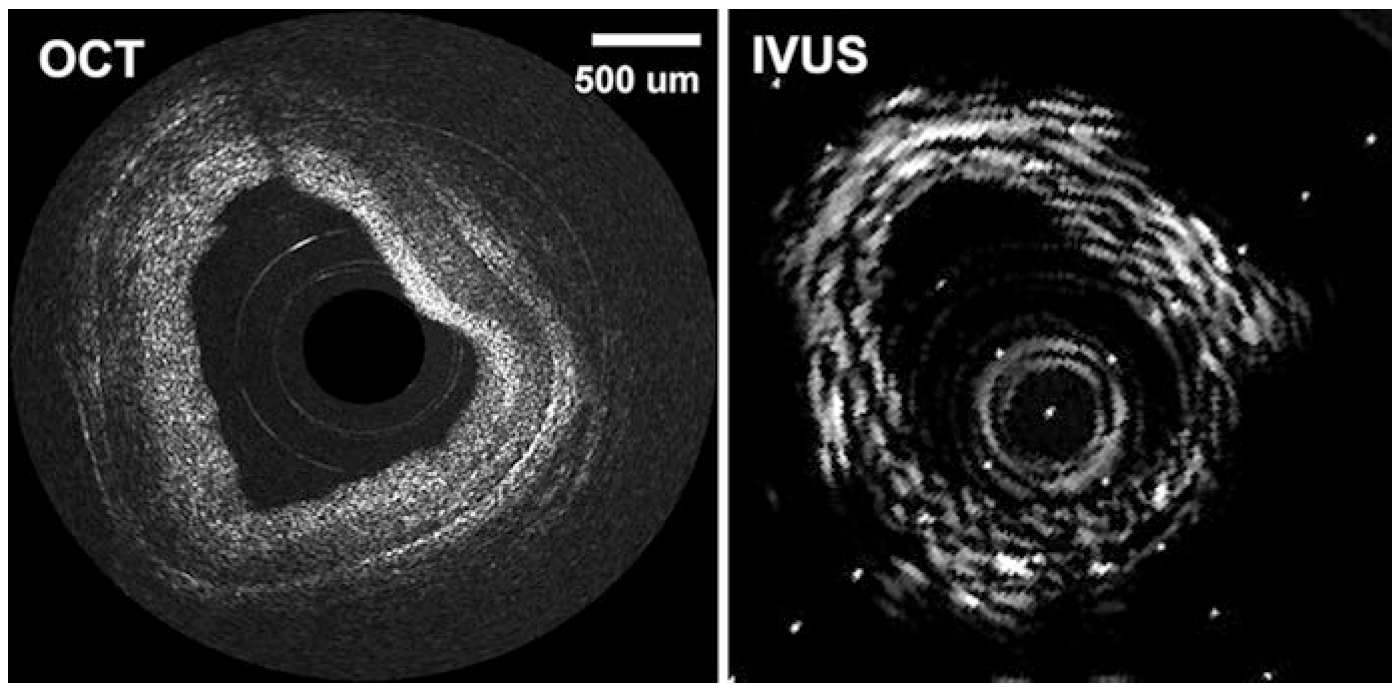
\includegraphics[width = \textwidth, keepaspectratio]{img/oct_intravascular_ultrasonido.png}
%	\caption[Comparación de OCT intravascular con ultrasonido]{Comparación de una imagen de OCT intravascular con ultrasonido (IVUS).}
%	\label{fig:oct_intravascular_ultrasonido}
%\end{figure}

%\subsubsection{Endoscopías y detección de cáncer con OCT}

%Por último, la OCT también ha sido empleada en el caso de la endoscopía. El primer estudio de endoscopía \invivo con imágenes de OCT fue realizado en 1997 \cite{Tearney1997, Sergeev1997}, un ejemplo de los resultados obtenidos por Tearney \emph{et al.} se muestra en la Fig.~\ref{fig:oct_endoscopia_conejo}. En la figura se observan las capas del esófago \emph{in vivo} de un conejo, en ella estructuras tales como la mucosa(m), submucosa(sm), mucosa interna (im), mucosa externa (om), serosa(s) y los tejidos de soporte vascular (a) pueden apreciarse. Los primeros estudios de endoscopía con imagen OCT en humanos fueron reportados por Sergeev \etal en 1997 \cite{Sergeev1997} y Feldchtein \etal en 1998 \cite{Feldchtein1998}, en donde se tomaron imágenes mediante  una sonda de barrido delantero en el canal de estándar. Estos estudios mostraron la utilidad de realizar OCT para imagen clínica de órganos tales como el esófago, la laringe, el estomago, la vejiga urinaria y el cuello uterino.


Por último, la OCT también ha sido empleada en el caso de la endoscopía. El primer estudio de endoscopía \invivo con imágenes de OCT fue realizado en 1997 \cite{Tearney1997, Sergeev1997}, en donde se obtuvieron los primeros resultados para el estudio del esófago de un conejo. Las imágenes de la OCT permitieron diferenciar de manera clara diferentes estructuras tales como la mucosa y la serosa. Los primeros estudios de endoscopía con imagen OCT en humanos fueron reportados por Sergeev \etal en 1997 \cite{Sergeev1997} y Feldchtein \etal en 1998 \cite{Feldchtein1998}, quienes mediante una sonda obtuvieron imágenes de membranas mucosas del esófago, la laringe, el estómago, la vejiga urinaria y el cuello uterino; mostrando así la utilidad de OCT en imagen clínica.

%\begin{figure}[ht!]
%	\centering
%	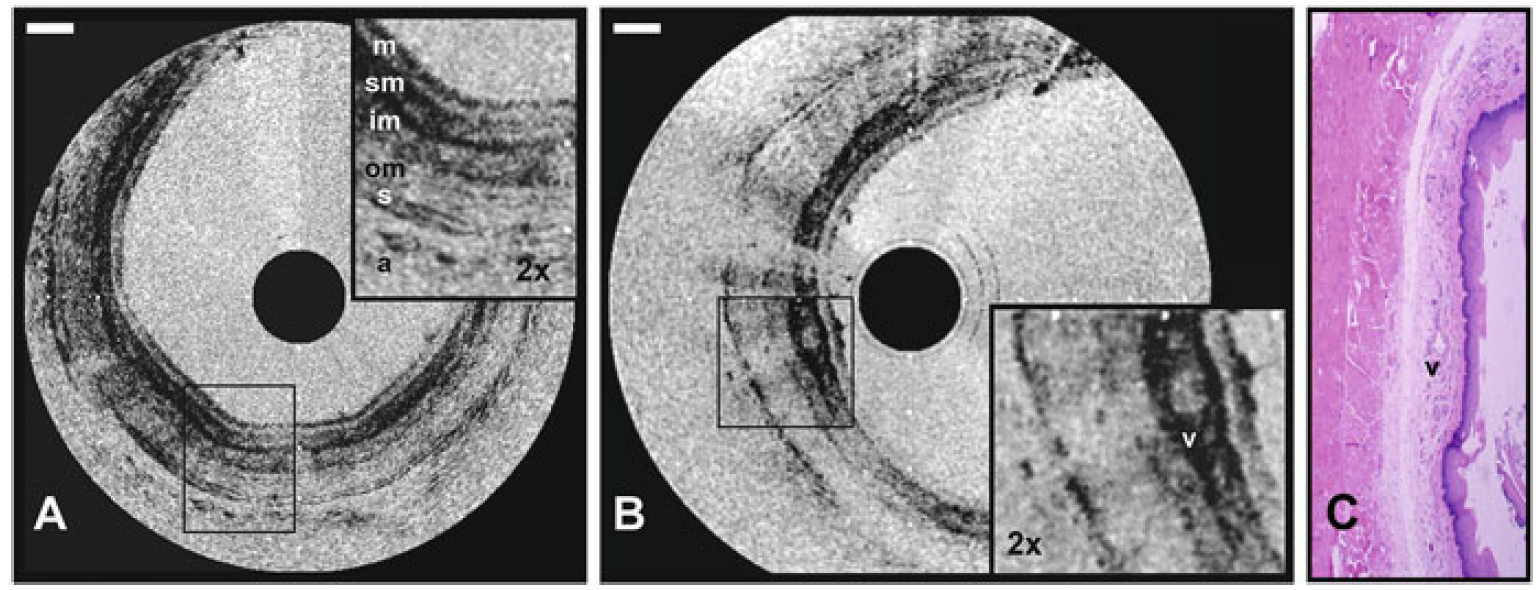
\includegraphics[width = \textwidth, keepaspectratio]{img/oct_endoscopia_conejo.png}
%	\caption[Endoscopía \emph{in vivo} del esófago de un conejo.]{Endoscopía \emph{in vivo} del esófago de un conejo. En la imagen (a) pueden observarse las capas del esófago, entre las que se aprecia: la mucosa(m), submucosa(sm), mucosa interna (im), mucosa externa (om), serosa(s) y los tejidos de soporte vascular (a). (v) es una vena que puede observarse en la submucosa. (c) histología. Escala $500um$. Tomada de Tearney \emph{et al.} \cite{Tearney1997}}
%	\label{fig:oct_endoscopia_conejo}
%\end{figure}

Dado el crecimiento de casos de cáncer en el esófago, estomago y colon, la endoscopía gastrointestinal tuvo una mayor atención, en contraste con esto, los estudios iniciales de OCT mostraron las ventajas de esta técnica para visualizar estructuras superficiales, ya que permite no solo ver las capas exteriores, sino que adicionalmente puede observar morfologías de tejidos bajo la superficie, permitiendo diferenciar patologías gastrointestinales, tales como el esógafo de Barret, los pólipos adenomatosos y el adenocarcinoma \cite{Bouma1999, Sergeev1997, Rollins1999, Jackle2000, Jackle2000_2, Sivak2000}. Los estudios de OCT para detección de cáncer son complejos, ya que los resultados de OCT deben ser comparados con técnicas estandarizadas tales como la biopsia que se ha convertido en un estándar en la detección de cáncer. El problema que tiene la OCT es que el contraste producido por las variaciones en las propiedades dispersivas de diferentes tejidos puede producir errores en las muestras tomadas dada la sensibilidad de OCT.

%\subsubsection{La tecnología del OCT en catéteres y endoscopios}

%El desarrollo de catéteres y endocopios ha sido fundamental para la implementación de OCT al interior del cuerpo \cite{Tearney1996, Tearney 1997_2}. La Fig.~\ref{fig:oct_cateter} muestra uno de los primeros sistemas de catéteres/endoscopios para OCT, el dispositivo posee una fibra óptica de modo único en un cable hueco rotatorio acoplado a una lente y a un microprisma que refleja la luz de radialmente. El haz es escaneado mediante la rotación del cable para generar una imagen transversa de la estructuras iluminadas. El diseño de este tipo de dispositivos para imagen mediante catéteres representa un desafío, ya que hay múltiples requerimiento tanto mecánicos, como ópticos y de biocompatibilidad que se deben abordar.

%\begin{figure}[ht!]
%	\centering
%	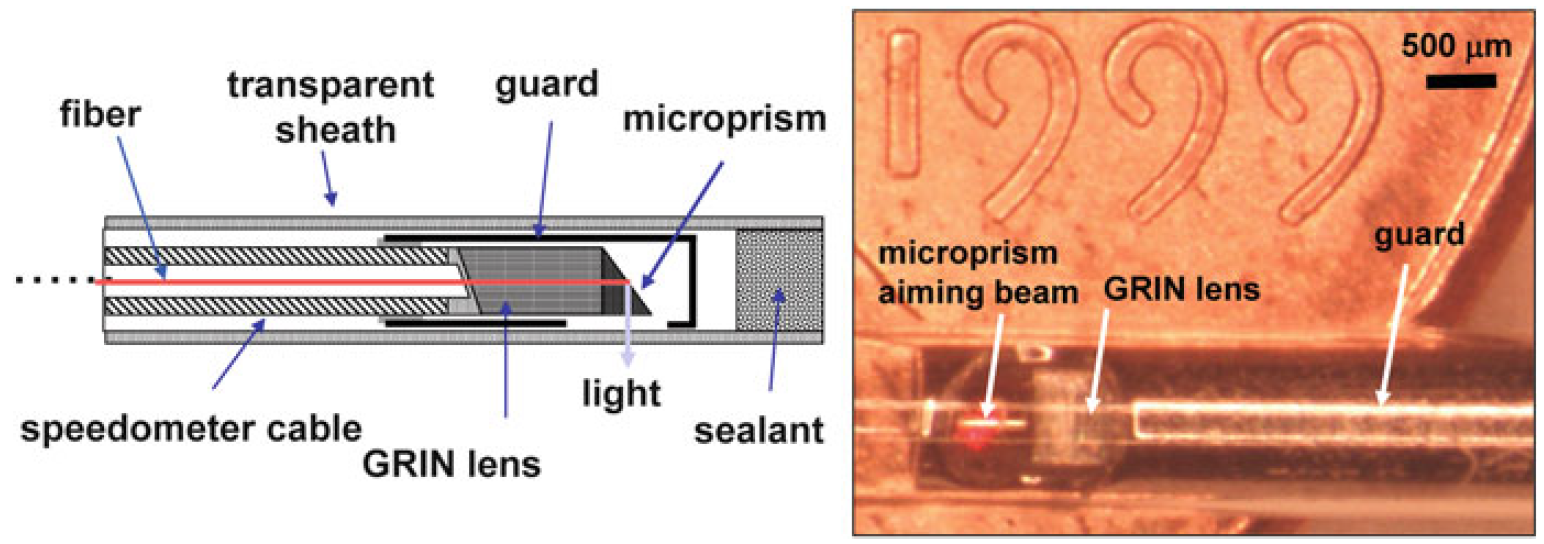
\includegraphics[width = \textwidth, keepaspectratio]{img/oct_cateter.png}
%	\caption[OCT mediante catéteres.]{Ejemplo de los primeros catéteres empleados para OCT.}
%	\label{fig:oct_cateter}
%\end{figure}

%
%Aunque OCT ha sido ampliamente estudiado y son constantes las nuevas publicaciones con propuestas, métodos, materiales y desarrollos, esta técnica aun presenta dificultades en su implementación. Un ejemplo de esto, es el escaneo lateral que debe realizarse para obtener las imágenes volumétricas
%
%La corrección del movimiento y la desviación producida por el escaneo son 
%
%El efecto que produce un muestro obliquo ha sido estudiado por 
%J. Walther, A. Krüger, M. Cuevas, and E. Koch. ``Effects of axial, transverse, and oblique sample motion in FD OCT in systems with global or rolling shutter line detector''. J. Opt. Soc. Am. A \textbf{25}(11), 2791-2802 (2008).
%
%
%
%
%Y han sido propiestas correcciones como
%M. Pircher, B. Baumann, E. Götzinger, H. Sattman, and C. Hitzenberger. ``Simultaneous SLO/OCT imaging of the human retina with axial eye motion correction''. Optics Express \textbf{15}(25), 16922-16932 (2007).
%
%S. Ricco, M. Chen, H. Ishikawa, G. Wollstein, J. Schuman, Correcting motion artifacts in retinal spectral domain optical coherence tomography via image registration. Med. Image Comput. Comput. Assist. Intervent. Miccai Proceedings \textbf{5761}, 100–107 (2009).
%
%B. Antony, M.D. Abramoff, L. Tang, W.D. Ramdas, J.R. Vingerling, N.M. Jansonius, K. Lee, Y.H. Kwon, M. Sonka, M.K. Garvin, Automated 3-D method for the correction of axial artifacts in spectral-domain optical coherence tomography images. Biomed. Opt. Exp. \textbf{2}, 2403–2416 (2011).
%
%
%
%Por otra parte, en OCT puede aparecer moteado (\textit{speckle}) causado por la dispersión que produce la muestra, aunque para OCT se han desarrollado algunos algoritmos de supresión de ruido, 

%Si bien OCT se ha expandido en la comunidad científica y médica, es de anotar que en el contexto científico Colombiano no se encuentra grupos de investigación vinculados a proyectos de desarrollo en áreas relacionadas con OCT. Por otra parte, las publicaciones internacionales por autores Colombianos que trabajen con OCT desde el punto de vista clínico también son escasas \cite{Hernandez2009,Homero2013}.

En general, dada la versatilidad y aplicabilidad de la OCT ha mostrado ser una técnica con altas posibilidades de implementación en diferentes áreas y aplicaciones de la medicina. Este documento presenta un marco teórico de los desarrollos y limitaciones que han surgido en la OCT con el fin de plantear un tema de investigación en esta área. Para dicho fin, el documento se encuentra organizado de la siguiente manera: en la Sección~\ref{sec:planteamiento_del_problema} se presenta el planteamiento del problema de investigación. En la Sección~\ref{sec:antecedentes_marco_teorico} se encuentran los antecedentes y marco teórico que detalla aspectos fundamentales a considerar sobre el desarrollo de la OCT. En la Sección~\ref{sec:objetivos} se presentará el objetivo general y los objetivos específicos que se espera completar con el trabajo de grado. La Sección~\ref{sec:metodologia} explicará en detalle los pasos propuestos para el desarrollo de las actividades y la realización de los objetivos específicos. La Sección~\ref{sec:cronograma} mostrará el cronograma planteado para el trabajo de grado, y posteriormente, se listarán los recursos necesarios para el desarrollo del trabajo de grado (Sección~\ref{sec:recursos}) y las referencias bibliográficas empleadas en este anteproyecto.

\section{Planteamiento del problema}
\label{sec:planteamiento_del_problema}

%En la implementación inicial de la OCT, conocida como OCT de primera generación o OCT en el dominio del tiempo [\textit{time-domain OCT}(TDOCT)], los datos en profundidad eran adquiridos mediante el desplazamiento axial del haz de referencia y posteriormente trasladando perpendicularmente el haz de escaneo. Sin embargo, hacia 1995 Fercher \etal \cite{Fercher1995} propusieron un nuevo método de medición cuyo funcionamiento era similar al de la OCT. La propuesta de Fercher consistía en medir el espectro de la luz, en lugar de tomar interferogramas a diferentes profundidades. El fundamento destrás de esta propuesta, es que el proceso de cambiar la distancia es equivalente a variar la longitud de onda, y se encuentran relacionados mediante una transformada de Fourier.



%En el sistema interferométrico sobre el cual se basa la OCT funciona a partir de una fuente blanca, haciendo uso del hecho de que la interferencia solo es producida en la región contenida dentro de la longitud de coherencia. Como se mencionó en la introducción, las imágenes volúmetricas son obtenidas en los siguientes pasos (Fig.~\ref{fig:scaningsystemoct}): primero se toman escaneos de manera axial para obtener el perfil de reflectividad en profundidad de la muestra, este proceso puede realizarse fácilmente a través del desplazamiento del espejo de referencia. Luego, se desplaza el haz objeto de manera lateral, es decir, en el plano $xy$ de la Fig.~\ref{fig:scaningsystemoct}. La interferencia es colectada por un foto detector, a continuación pasa por una etapa de adquisición de datos (DAQ) y finalmente los datos son transferidos hasta el computador.

%La Fig.~\ref{fig:scaningsystemoct} 

En la implementación inicial de la OCT, la información en profundidad es obtenida mediante desplazamientos axiales del haz de referencia que son producidos por actuadores tales como piezoeléctricos, así como lo indica la Fig.~\ref{fig:scaningsystemoct}. En ese sistema de OCT, la luz producida por la fuente viaja mediante una fibra óptica hasta llegar a un acoplador, en donde se divide por dos caminos diferentes; uno de ellos viaja directamente hasta el espejo de referencia que tiene la posibilidad de desplazarse en sentido axial. Posteriormente, el haz reflejado por el espejo regresa hacia la fibra óptica. El segundo haz es dirigido hacia un espejo de escaneo cuya función es desviar la luz que es proyectada en la muestra de manera controlada. Mediante este sistema, la porción de luz que sea reflejada por la muestra hacia la fibra óptica volverá a incorporarse al sistema óptico regresando hasta el acoplador. La información de los dos haces juntos llega entonces hasta un sensor que se encarga de obtener la señal interferométrica. El sensor transfiere los datos a un sistema de adquisición de datos (DAQ) y finalmente las señales son enviadas hasta el computador. 

La información volumétrica requiere que el haz proyectado hacia la muestra sea desplazado de manera lateral en dos direcciones, procedimiento que se ha realizado a través del uso de sistemas microelectromecánicos (MEMS) que permiten la inclinación controlada del haz, y por tanto el desplazamiento de éste sobre la muestra \cite{Zara2003,Jung2006,Aguirre2007}. El espejo de escaneo se encarga de mover el haz sobre el plano imagen produciendo imágenes bidimensionales de planos $xy$ a profundidades $z$ específicas, a este tipo de imagen se le conoce como \emph{en-face}. Una de las limitaciones de los sistemas para OCT surge justamente en la implementación del sistema de escaneo, ya que hay errores producidos no solo por la instrumentación sino por la misma muestra. 

\begin{figure}[th!]
	\centering
	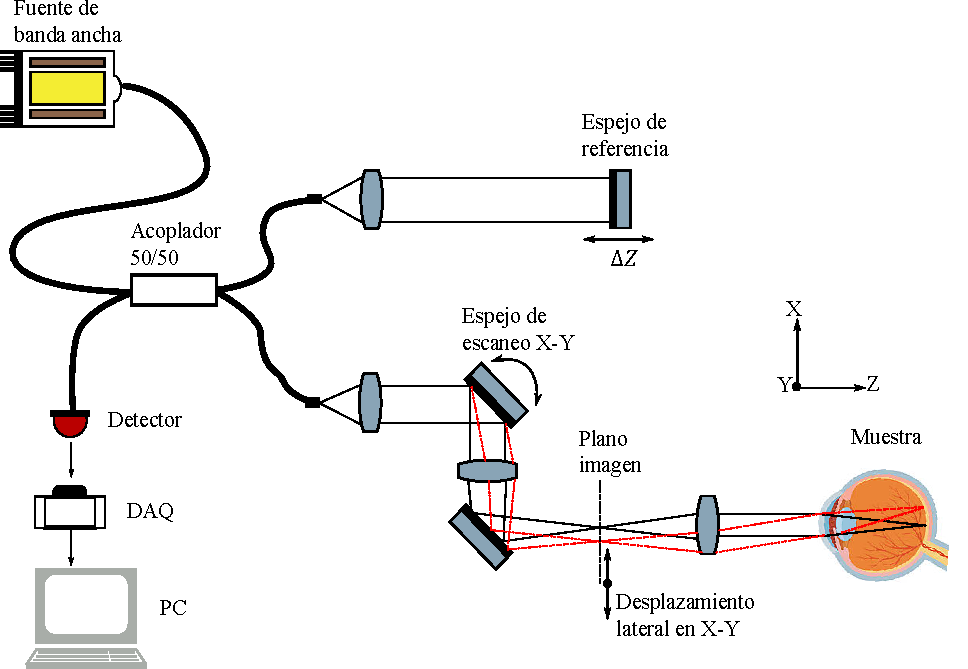
\includegraphics[width=0.7\linewidth]{img/scaning_system_oc.pdf}
	\caption{Sistema de escaneo para la OCT.}
	\label{fig:scaningsystemoct}
\end{figure}


Desde el punto de vista instrumental, algunos espejos de escaneo emplean sistemas de control retroalimentados tales como PID que se encargan del desplazamiento y control del sistema \cite{xie2004}, sin embargo, este tipo de control en lazo cerrado puede tener la falencia de enviar voltajes fluctuantes  que producen desviaciones, y pueden ser causados o bien por las constantes del controlador o por desplazamientos repentinos producidos por el paciente. Otros sistemas basados en MEMS \cite{Strathman2014} requieren voltajes AC para producir respuestas lineales, sin embargo, fluctuaciones en la frecuencia o en la amplitud del voltaje suministrado al actuador producen respuestas diferentes a la esperada. Adicionalmente, mientras se realizan los escaneos axiales, el espejo de escaneo se mueve a velocidad constante en las dos direcciones, por lo tanto hay una dirección con una velocidad menor (\emph{slow-axis}) y otro con una mayor velocidad (\emph{fast-axis}), esto hace necesario una corrección del movimiento en las imágenes de OCT obtenidas \cite{Yun2004, Pierce2005, Drexler2015}. En cuanto a la muestra que es tomada en pacientes, existen diferentes movimientos involuntarios que no pueden ser controlados, tales como la contracción muscular causada por la respiración o el parpadeo, así como cualquier movimiento que el paciente pudiera realizar mientras el sistema se encuentra en proceso de escaneo.

%Las limitaciones mencionadas anteriormente, si bien pueden no tener una incidencia directa sobre la reconstrucción de la reflectividad producida por la muestra, si tiene un impacto directo en la reconstrucción de la fase, a estos errores en la fase las denominaremos corrupciones de fase. Ahora bien, como se ha mencionado, la OCT se basa en la medición de la interferencia causada entre la luz dispersada por una muestra y un haz de referencia \cite{Huang1991}. Bajo este principio, la OCT es capaz de medir no solo la amplitud del campo reflejado por la muestra, sino que también puede medir su fase; tomando esto en cuenta, numerosas extensiones de OCT que emplean principalmente la fase han surgido bajo el nombre de \emph{phase resolved OCT}, entre estas sobresalen: OCT Doppler \cite{Chen1999}, microangiografía óptica \cite{Wang2010}, elastografía óptica de coherencia \cite{Ruikang2007} y OCT magnetomotriz \cite{Oldenburg2005}. En OCT Doppler por ejemplo, es común encontrar aplicaciones de flujometría, en el cual el sistema interferométrico de la OCT permite la detección de saltos en la fase causados por el movimiento de los centros dispersores en la muestra que no es posible observar con la amplitud. Mediante este proceso, es posible seguir el movimiento de los centros dispersores y cuantificar su velocidad de flujo \cite{Chen1999}. 

Ahora bien, como se ha mencionado, la OCT se basa en la medición de la interferencia causada entre la luz dispersada por una muestra y un haz de referencia \cite{Huang1991}. Bajo este principio, la OCT es capaz de medir no solo la amplitud del campo reflejado por la muestra, sino que también puede medir su fase. Los errores en la toma de datos que pueden ser producidos por el sistema de escaneo, así como el paciente, si bien pueden no tener una incidencia directa sobre la reconstrucción de la reflectividad producida por la muestra, si tiene un impacto directo en la reconstrucción de la fase; a estos errores en la fase los denominaremos corrupciones de fase. Numerosas extensiones de OCT que emplean principalmente la fase han surgido bajo el nombre de \emph{phase resolved OCT}, entre estas sobresalen: OCT Doppler \cite{Chen1999}, microangiografía óptica \cite{Wang2010}, elastografía óptica de coherencia \cite{Ruikang2007} y OCT magnetomotriz \cite{Oldenburg2005}. En OCT Doppler por ejemplo, es común encontrar aplicaciones de flujometría, en el cual el sistema interferométrico de la OCT permite la detección de saltos en la fase causados por el movimiento de los centros dispersores en la muestra que no es posible observar con la amplitud. Mediante este proceso, es posible seguir el movimiento de los centros dispersores y cuantificar su velocidad de flujo \cite{Chen1999}. 

Otro problema que es común en los datos adquiridos mediante OCT es el moteado (\textit{speckle}), el cual cumple una doble función ya que puede aportar información de la muestra o puede surgir como ruido \cite{Schmitt1999,Mariampillai2008}. En OCT el moteado como ruido surge cuando la señal que se registra en el detector posee información de la interferencia que se produce entre la luz dispersada por centros dispersores cercanos al área de escaneo, y en lugar de portar información sobre la muestra, degradan la calidad de la señal que se registra y dificultan su interpretación. En OCT existen diferentes técnicas de reducción de ruido multiplicativo \cite{Hughes2009,Szkulmowski2012,Aum2015}, aunque tienen la desventaja de poseer altos tiempos de procesamiento, y en algunos casos, requieren una imagen con bajo coeficiente señal-ruido para su correcto funcionamiento \cite{Fang2012}.

La propuesta para este trabajo de grado consiste en facilitar la interpretación y procesamiento de datos provenientes de OCT, mediante la implementación de técnicas de posprocesamiento que permitan mejorar la calidad de los datos adquiridos.
	\section{Antecedentes y marco teórico}
\label{sec:antecedentes_marco_teorico}
\subsection{Tomografía óptica de coherencia}

En lo últimos años han aparecido nuevas técnicas para la toma de imágenes en múltiples disciplinas científicas, entre ellas destacan por su alta actividad de investigación, la formación de imágenes biomédicas, impulsado principalmente por el constante desarrollo de dispositivos para telecomunicaciones que han permitido la producción de instrumentos electromagnéticos de alto desempeño a costos relativamente bajos. Como consecuencia de esto, múltiples técnicas para el escaneo materiales altamente dispersivos, como los tejidos biológicos han sido creadas. De estas técnicas surge la tomografía, que es particularmente interesantes por su potencial para realizar imágenes que ayudan al diagnóstico médico a través de exámenes \emph{no invasivos}. La tomografía en general se basa en la creación de ``cortes''  de objetos tridimensionales, que en conjunto generan una imagen en dos o tres dimensiones de la muestra en cuestión. \emph{La OCT es una técnica no invasiva de imagen tridimensional capaz de producir imágenes con alta resolución lateral y axial a través de muestras dispersivas e inhomogéneas, tales como los tejidos biológicos} \cite{Tomlins}. En sus inicios, las técnicas de OCT se basaron en medidas de profundidad de baja coherencia en el dominio temporal con un interferómetro de luz blanca. La posibilidad de emplear interferómetros de luz blanca para la formación de imágenes tridimensionales en tejidos biológicos fue liderada por Huang \etal en 1991 \cite{Huang1991}, quienes propusieron emplear reflectometría de baja coherencia en sistemas biológicos. Su sistema de OCT se basa en múltiples escaneos de una serie de ubicaciones laterales y axiales para proveer un mapa de sitios o lugares en donde la muestra refleja luz. Una de las características más importantes de esta nueva técnica, es que a diferencia de la microscopía confocal, en donde la resolución longitudinal depende de la apertura numérica, en OCT la resolución solo está limitada por la longitud de coherencia de la fuente de luz, por consiguiente, OCT puede tener alta resolución en profundidad aun si la apertura del sistema es pequeña.

\subsection{El papel de la OCT en imagen médica}

La OCT tiene diversos aspectos que son comunes al ultrasonido y a la microscopía. Por un lado, la resolución en imágenes de ultrasonido de alta resolución, se encuentra en el rango típico de $0.1$ hasta $1mm$ y dependerá de la frecuencia de la onda de sonido que se emplee, los valores típicos para la frecuencia varían entre los $3$ y $40MHz$ \cite{Szabo}. Sin embargo, en este rango de frecuencias es difícil emplear las ondas de sonido en tejidos, ya que éstos además de ser altamente dispersivos, atenúan fuertemente las ondas en unos pocos milímetros. Por otro lado, algunas ramas de la microscopía poseen una alta resolución en imagen de tejidos, por ejemplo, la microscopía confocal, cuya resolución es de alrededor de $1\mu m$ o inclusive menor. En la microscopía confocal, la resolución está limitada por la difracción, relacionada a su vez con la apertura numérica del sistema; y su capacidad de producir imagen se encuentra influenciada principalmente por la degradación de la luz en dispersiones no deseadas, lo que produce un bajo contraste en la señal a medir \cite{Pawley}. 

La OCT por su lado, llena un vacío de resolución entre el ultrasonido y la microscopía, ya que el rango en el cual se mueve la OCT varía entre $1$ y $15 \mu m$, aproximadamente $100$ veces más fino que el ultrasonido, como se presenta en la Fig.~\ref{fig:OCT_Ultrasound_microscopy}. La principal limitación en OCT se encuentra en que la luz es altamente dispersada por muchos tejidos, lo que limita la profundidad de penetración a $\sim 2mm$ en muchos casos.
%Mientras que una de sus principales ventajas está en su fácil integración en instrumentos médicos, tales como catéteres, endoscopios, laparoscopios o incluso, agujas quirúrgicas que permite hacer imagen de órganos, o incluso, tejidos sólidos en el cuerpo.

\begin{figure}[ht!]
	\centering
	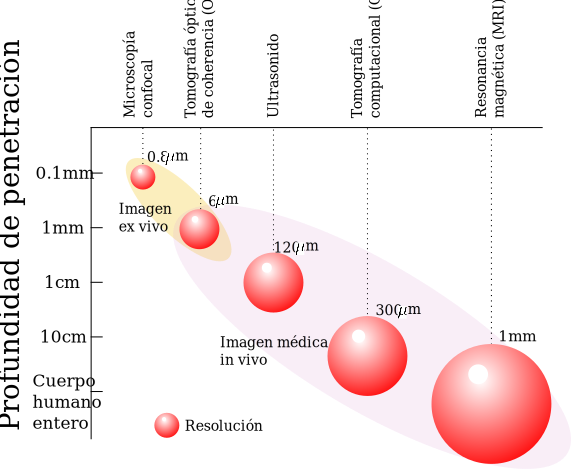
\includegraphics[width = 0.7\textwidth, keepaspectratio]{img/Carlos_oct_resolucion}
	\caption{Comparación de la resolución contra la profundidad de penetración de diferentes modalidades de imagen médica.}
	\label{fig:OCT_Ultrasound_microscopy}
\end{figure}


La OCT es análoga al ultrasonido con la diferencia de emplear luz en lugar de sonido, su principio básico se centra en medir la magnitud y el tiempo de retraso (``eco'') que producen las ondas al llegar a la muestra, de forma que las retrodipersiones o retroreflecciones en diferentes distancias permite determinar el tamaño y reconstruir microestructuras \cite{Szabo}. Como la velocidad del sonido es de alrededor de $1300m/s$, el ultrasonido ha impulsado la creación de sensores y métodos de sensado que permitan una alta tasa de recepción de información, lo que a su vez ha incentivado el desarrollo de equipos para OCT, en especial si se considera que la luz viaja a $3\times 10^8 m/s$ y que las tasas de recepción de datos deben de ser mayores. Una de las principales ventajas de la analogía OCT/ultrasonido se encuentra en su fácil integración en instrumentos médicos, tales como catéteres, endoscopios, laparoscopios o incluso, agujas quirúrgicas que permite hacer imagen de órganos o tejidos sólidos \invivo en el cuerpo humano~\cite{Tearney1996, Tearney1997_2}.

%La OCT es análoga al ultrasonido, con la diferencia de emplear luz en lugar de sonido. El principio básico de la OCT, es medir la magnitud y el retraso de las retrodipersiones o retroreflecciones de la luz en microestructuras en tejidos, de forma que el tamaño de las microsestructuras puede determinarse a través de la medida del tiempo que tarda el ``eco'' del sonido o la luz en viajar diferentes distancias. El desarrollo de equipos para tratamientos con ultrasonido a su vez ha posibilitado la creación de equipos de bajo costo para OCT, en especial si se considera que la velocidad del sonido es de alrededor de $1300m/s$, mientras que la luz viaja a $3\times 10^8 m/s$. Una de las principales ventajas de la analogía OCT/ultrasonido se encuentra en su fácil integración en instrumentos médicos, tales como catéteres, endoscopios, laparoscopios o incluso, agujas quirúrgicas que permite hacer imagen de órganos o tejidos sólidos \invivo en el cuerpo.

\subsection{Los inicios de la OCT}

%La propuesta de la técnica de OCT surgió hacia el año 1991 por Huang \etal \cite{Huang1991}, sus primeras pruebas fueron realizadas \emph{ex vivo} en la retina y la arteria coronaria. Huang \etal proponen una técnica análoga al ultrasonido, pero que en lugar de emplear ondas de sonido, emplea luz para realizar reconstrucciones tridimensionales a partir de escaneos bidimensionales, a esta técnica la denominarían tomografía óptica de coherencia, y se basa esencialmente en el empleo de un interferómetro de luz blanca. Con los resultados obtenidos por Huang \etal la OCT se ha posicionado como una de las más grandes aplicaciones emergentes para el diagnóstico oftalmológico e intravascular.

La propuesta de OCT surgió hacia el año 1991 por Huang \etal \cite{Huang1991}, sus primeras pruebas fueron realizadas \exvivo en la retina y la arteria coronaria, y desde estos resultados pudo verse la utilidad de OCT para el diagnóstico oftalmológico e intravascular, áreas en las que ha tenido grandes avances. El ojo humano puede ser analizado ópticamente, es decir, es posible implementar técnicas para observar de manera directa la zona interior del ojo, lo que ha impulsado el uso de métodos de imagen en oftalmología; muchos de los primeros estudios realizados con OCT fueron basados en el ojo humano. Las primeras imágenes \invivo de la retina fueron obtenidas de manera independiente por Fercher \etal \cite{Fercher1993} y Swanson \etal \cite{Swanson1993} en 1993. Estos resultados conllevaron a que en la década de los 90 se diera un alto uso de OCT para el monitoreo, seguimiento, detección y diagnosis de diferentes enfermedades, entre las cuales destaca: enfermedades maculares \cite{Puliafito1995}, incluyendo agujeros maculares \cite{Hee1995_2} y edemas maculares \cite{Hee1995},  coriorretinopatía serosa central \cite{Hee1995_3}, y degeneraciones maculares asociadas a la edad y a la neovascularización coroidal \cite{Hee1995_4}. Un ejemplo de monitoreo con OCT, está en el espesor de las capas de fibra del nervio retinal, el cual es un indicador de glaucoma, y que puede cuantificarse en ojos normales y con glaucoma. Mediante una correlación con medidas convencionales de la estructura y función del nervio óptico, es posible encontrar focos de glaucoma, trabajo realizado también a partir de la OCT en 1995 por Schuman \etal \cite{Schuman1995}.

La alta sensibilidad de la OCT permite producir imagen de estructuras tales como la retina, que poseen un bajo índice de dispersión de la luz, sin embargo, la mayor parte de las aplicaciones que emplean OCT requieren la captura de imágenes en tejidos que no son transparentes y además, son altamente dispersivos. En estos casos, es cuando la sensibilidad del método se vuelve relevante, ya que como la señal es fuertemente atenuada por la dispersión, la sensibilidad es quien determina la profundidad hasta la cual se puede conseguir imágenes \cite{Drexler2015}. Las primeras imágenes de tejidos diferentes al ojo, fueron posibles mediante el estudio de la influencia de la longitud de onda en la dispersión de la luz, en done se obtuvo que longitudes de onda más largas que el visible, reducen la dispersión producida por las muestras biológicas e incrementa la profundidad de penetración de la imagen \cite{Brezinski1996, Schuman1995}. Uno de los primeros estudios del efecto de la longitud de onda sobre las reconstrucciones con OCT fue realizado por Brezinski \etal \cite{Brezinski1996}, quienes realizaron una comparación de imágenes capturadas a $850$ y $1300nm$ \exvivo en una epiglotis humana. La imagen tomada a $1300nm$ mostró una mayor penetración puesto que los principales absorbentes en la mayor parte de los tejidos son la melanina y la hemoglobina, los cuales poseen una alta absorción en el visible y el infrarojo cercano \cite{Parsa1989}, mientras que la absorción del agua se convierte en dominante para mayores longitudes de onda, alrededor de los $1800-2000nm$. Por otro lado, en la mayoría de los tejidos, la dispersión en las longitudes de onda del infrarrojo cercano es uno o dos órdenes de magnitud mayores que la absorción, y la dispersión disminuye para longitudes de onda más grandes.

%\begin{figure}[ht!]
%\centering
%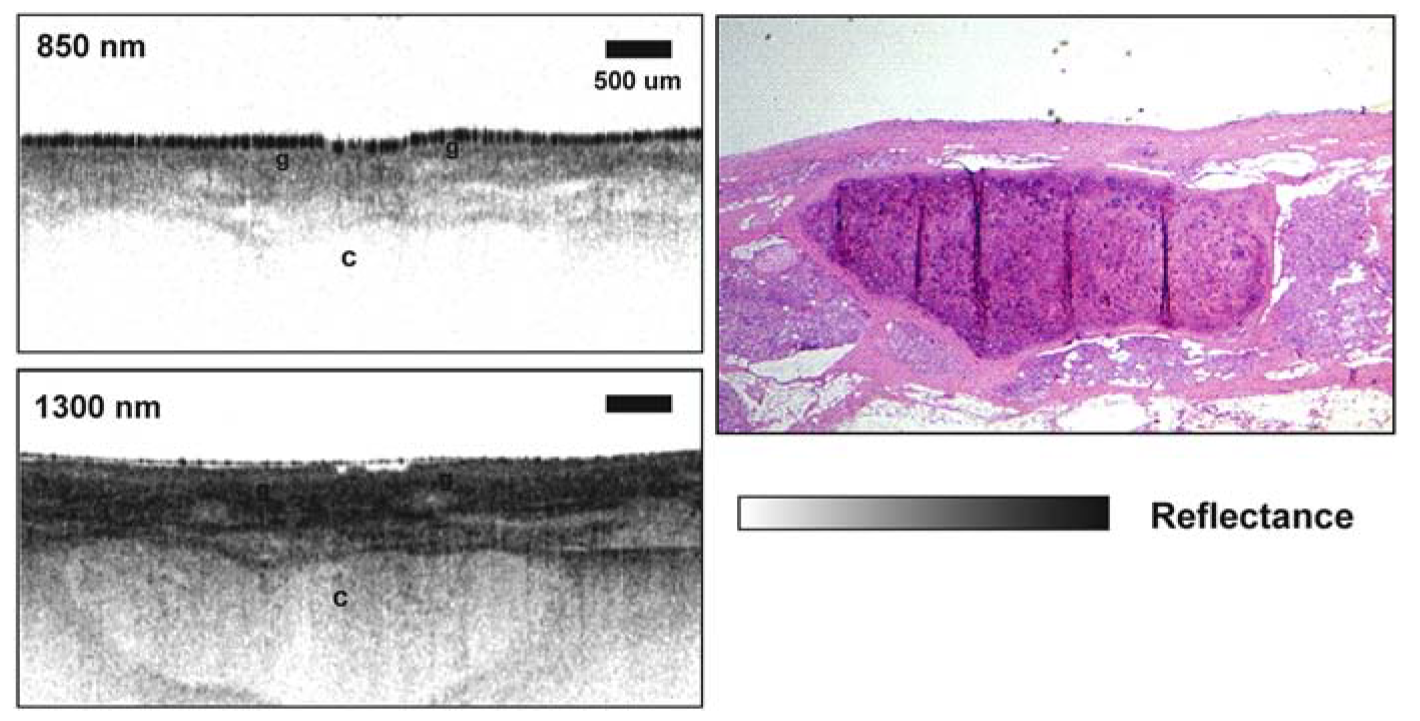
\includegraphics[width = \textwidth, keepaspectratio]{img/oct_longitudes_multiples.png}
%\caption[OCT empleando diferentes longitudes de onda.]{Profundidad de penetración de la OCT en diferentes longitudes de onda. Comparación de la atenuación producida por diferentes longitudes de onda en OCT, visualmente se aprecian más detalles cuando se emplea una longitud de onda de $1300nm$ que con $850nm$. Tomado de \cite{Brezinski1996}.}
%\label{fig:oct_longitudes_multiples}
%\end{figure}

Muchos estudios iniciales de la OCT se realizaron \exvivo en especímenes quirúrgicos, estos estudios fueron útiles para definir las estructuras que serían posibles de observar usando OCT \cite{Brezinski1996} y compararlo con la histología \footnote{estudio de la composición, estructura y características de los tejidos orgánicos de los seres vivos}. El estudio de la correlación entre las imágenes \exvivo de la  OCT y la histología se extendió a estudios hasta de enfermedades gastrointestinales \cite{Izatt1996, Tearney1997, Kobayashi1998, Pitris2000}, biliares \cite{Tearney1998}, en el aparato reproductor femenino \cite{Pitris1999}, pulmonares \cite{Pitris1998} y urinarias \cite{Tearney1997}.


\subsection{OCT: esquema}
\label{sec:OCT_Esquema}

\emph{La OCT es una técnica interferométrica que se basa en la interferencia de un campo óptico de banda ancha, es decir, que recoge múltiples longitudes de onda, el cual se divide y posteriormente se combina, produciendo interferencia únicamente en la región del espacio en el cual la diferencia de camino óptico se encuentra dentro de la longitud de coherencia} \cite{Fercher}. Un esquema típico de OCT se muestra en la Fig. \ref{fig:OCT_Scheme}. 

\begin{figure}[ht!]
	\centering
	\includegraphics[width = 0.5\textwidth, keepaspectratio]{img/Carlos_oct_Scheme}
	\caption{Esquema básico de la OCT, un interferómetro de Michelson se emplea para producir interferencia de baja coherencia entra el haz objeto y referencia.}
	\label{fig:OCT_Scheme}
\end{figure}

El esquema de la OCT se basa esencialmente en un interferómetro de Michelson que funciona de la siguiente forma: Primero un haz que proviene de una fuente viaja a través de un divisor de haz. Los haces divididos a su vez van por dos caminos diferentes, la porción del haz de referencia se refleja en un espejo, mientras que la otra porción del haz es enviada hacia la muestra, en donde se refleja desde diferentes profundidades al interior de la muestra. \emph{Como el haz posee una banda ancha, la interferencia entre el campo óptico de referencia y el que es reflejado por la muestra solo puede ser observado cuando ambos brazos tengan diferencias de camino óptico que se encuentren dentro de la longitud de coherencia del haz. Por consiguiente, la resolución axial de un sistema de OCT está determinado por la coherencia temporal de la fuente de luz}. En OCT, la longitud de coherencia $l_c$ se define como:

%Si la diferencia de camino óptico entre ambos brazos se encuentra dentro de la longitud de coherencia, se define el tamaño de ida y vuelta de longitud de coherencia $l_c$  como:

\begin{equation}
	\label{eq:l_c}
	l_c = \frac{2\ln 2}{\pi} \frac{\bar{\lambda}}{\Delta \lambda},
\end{equation}

\noindent donde $\bar{\lambda}$ es la longitud de onda central y $\Delta \lambda$ es el ancho del espectro (banda), $l_c$ indica la condición para la cual es posible obtener interferencia y por tanto la distancia axial mínima que puede medirse en OCT. \emph{Los objetos aparecen cuando se dan cambios precipitados en el índice de refracción entre profundidades o capas cercanas en la muestra, y se manifiestan como picos de intensidad en el patrón de interferencia}, nótese que la intensidad medida es aquella que proviene de la retrodispersión causada por la muestra. Debido a que el espectro es ancho, otra posibilidad de medir la información de profundidad en la muestra, es a través de las transformadas de Fourier, realizando mediciones sobre el dominio de las frecuencias y transformando el espectro de salida. En este caso, el haz de referencia permanece en una posición fija y las componentes frecuenciales de la OCT se detectan mediante un espectrómetro \cite{Drexler2015,Brezinski2005}.

En OCT pueden realizarse escaneos bidimensionales si no se modifica la diferencia de camino, o escaneos tridimensional a través de la medición de diversas profundidades en la muestra, que pueden ser realizadas mediante escaneos laterales del haz en una o dos direcciones ortogonales. Valores típicos de escaneos para profundidad pueden ir en $500$ profundidades distribuidas en una distancia de $3mm$ \cite{Tomlins}. Si el medio es turbio, las profundidades obtenidas en la literatura han sido entre $1$ y $3mm$, empleado longitudes de onda entre $800$ y $1300nm$ \cite{Drexler2015}.

Por último, algunas propiedades que cabe resaltar sobre OCT son las siguientes:
\begin{itemize}
	\item Alta resolución en imagen de profundidad.
	\item Resolución en profundidad, con distancias que van desde $1\mu m$ hasta $5mm$.
	\item Alta sensibilidad, permitiendo la captura de muestras poco dispersivas incluso en medios turbios.
	\item OCT no es una técnica invasiva, que posibilita su uso \invivo e \emph{in-situ}.
\end{itemize}

\subsection{Interferometría de baja coherencia}

Considere un intereferómetro de Michelson, como se muestra en la Fig.~\ref{fig:OCT_Scheme}, ese interferómetro es iluminado con una fuente de banda ancha, cuyo campo eléctrico $E_i$ puede expresarse en forma compleja como
\begin{equation}
	E_i(k,\omega) = s(k,\omega) e^{i(kz - \omega t)},
\end{equation}
donde $s(k,\omega)$ es la amplitud del campo eléctrico expresado como una función del número de onda $k = 2\pi /\lambda$ y de la frecuencia angular $\omega = 2\pi \nu$, que representan respectivamente la dependencia espacial y temporal de cada una de las componentes del espectro del campo con longitud de onda $\lambda$. La frecuencia y la longitud de onda se encuentran vinculadas por el índice de refracción del medio $n$ y la velocidad de luz en el vacío $c$, $\lambda \nu = c / n(\lambda)$, en medios dispersivos el índice de refracción depende de la longitud de onda. Se asume que el divisor de haz produce una división del campo incidente en dos componentes cada una con la mitad de la intensidad total, y adicionalmente es acromático. De los dos haces producidos por el divisor de haz, al que es reflejado cuando llega al divisor se le denota haz referencia, mientras que el que es refractado por el divisor haz objeto. El haz de referencia se propaga una distancia $z_R$ y nuevamente es reflejado por un espejo situado en $z = z_R$, el espejo de referencia tiene una reflectividad $r_R$ y la intensidad que refleja es $R_R = |r_R|^2$, finalmente, el haz reflejado regresar hasta el divisor de haz. 

El haz objeto por su parte, se propaga hasta llegar a la muestra. La muestra está caracterizada por tener una reflectividad de campo eléctrico dependiente de la profundidad $r_S(z_S)$, donde $z_S$ es la profundidad en la muestra medida desde el divisor de haz. En general, $r_S(z_S)$ es una función compleja que informa no solo la amplitud de la onda reflejada por la muestra, sino que además indica los cambios de fase que la onda puede experimentar. Adicionalmente, en el caso de especímenes biológicos, se trata de una función que refleja el cambio continuo del índice de refracción de los tejidos biológicos. Sin embargo, para entender el fenómeno de reflexión en la muestra, se asume que hay una serie de $N$ reflectores ubicados a lo largo de la muestra \footnote{Hay diferentes tratamientos que se basan en sistemas discretos y continuos, el último caso puede consultarse de manera detallada en \cite{Brezinski2005,Fercher}.}, de la siguiente forma, 

\begin{equation}
	r_S(z_S) = \sum_{n=1}^{N} r_{S_n} \delta[(z_S - z_{S_n})],
\end{equation}

\noindent donde $r_{S_1}, r_{S_2}, ..., r_{S_n}$ es el coeficiente de reflexión de campo eléctrico del $n$-simo reflector y $ z_{S_1}, z_{S_2}, ..., z_{S_n}$ es la distancia del $n$-simo reflector con respecto al divisor de haz. La intensidad reflejada por cada uno de los $n$ reflectores es $R_{S_n} = |r_{S_n}|^2$. \emph{El objetivo de OCT es poder identificar la función $\sqrt{R_{S}(z_S)}$ a través de medidas de interferométricas de baja coherencia}, lo que es la reflectividad de cada una de las profundidades en la muestra en estudio.



Luego de que el haz objeto y el haz referencia regresan al divisor de haz, el campo eléctrico reflejado corresponde a $E_R = \frac{E_i}{\sqrt{2}}r_Re^{i2kz_R}$ y $E_S = \frac{E_i}{\sqrt{2}} \sum_{n=1}^{N}r_{S_n} e^{i2kz_{S_n}}$ respectivamente. El factor exponencial surge por el cambio de fase que se produce durante la propagación, y la función $\delta$ del haz objeto ha sido incluida en el cambio de fase que se produce en la distancia $z_{S_n}$. Estos dos campo regresan hasta el divisor de haz y luego de atravesarlo tienen la mitad de su intensidad inicial, siguiendo su recorrido hasta llegar al detector, en donde se tiene la interferencia entre ellos $I(k,\omega)$, dada por

\begin{equation}
	I(k,\omega) = \frac{1}{2}|E_R+E_S|^2 = (E_R + E_S)(E_R + E_S)^{\ast},
\end{equation}

\noindent donde $^{\ast}$ representa la operación complejo conjugado. Si el patrón de interferencia $I(k,\omega)$ es registrado por un fotodetector, la fotocorriente que en este se produce es proporcional a la intensidad del patrón de interferencia multiplicado por un factor de respuesta propio del detector $I_D(k, \omega) = \rho \langle I(k, \omega) \rangle$, donde $\rho$ es el factor de respuesta del sensor y $\langle \cdot \rangle$ es la integración sobre el tiempo de respuesta. Reemplazando los valores anteriores, se puede expresar la corriente sensada por el detector como

\begin{equation}
\label{eq:Id}
	I_D(k, \omega) = \frac{\rho}{2} \bigg\langle \bigg| \frac{s(k, \omega)}{\sqrt{2}} r_R e^{i(2kz_R-\omega t)} + \frac{s(k, \omega)}{\sqrt{2}} \sum_{n=1}^{N} r_{S_n} e^{i(2kz_{S_n} - \omega t)} \bigg|^2 \bigg\rangle.
\end{equation}

Nótese que si se expande la Eq.~\ref{eq:Id}, los términos que son dependientes de $\omega$ se anulan y la expresión final es independiente del tiempo, esto tiene sentido si se considera que la frecuencia de la onda $\nu$ es mucho mayor que el tiempo de respuesta del detector. La Eq.~\ref{eq:Id} puede expresarse como

%La expresión simplificada de la Eq.~\ref{eq:Id} es
%
%\begin{align}
%\label{eq:ID_2}
%%	I_D(k) &= \frac{\rho}{4}\left[ S(k) (R_R + R_{S1} + R_{S2} + ...) \right] \notag \\
%	& + \frac{\rho}{4} \left[ S(k) \sum_{n=1}^{N} \sqrt{R_R R_{S_n}} \left( e^{i2k(z_R-z_{S_n})} + e^{-i2k(z_R-z_{S_n})} \right) \right] \\
%	& + \frac{\rho}{4} \left[ S(k) \sum_{m\neq n=1}^{N} \sqrt{R_{S_n}R_{S_n}} \left( e^{i2k(z_{S_n}-z_{S_m})} + e^{-i2k(z_{S_n}-z_{S_m})} \right) \right], \notag
%\end{align}
%
%\noindent donde $S(k) = \langle |s(k,\omega)|^2 \rangle$, que es la dependencia de $\lambda$ de la fuente. La Eq.~\ref{eq:ID_2} puede expresarse como

\begin{align}
\label{eq:ID_fin}
	I_D(k) &= \frac{\rho}{4}\left[ S(k) (R_R + R_{S1} + R_{S2} + ...+R_{Sn}) \right] \notag \\
	& + \frac{\rho}{2} \left[ S(k) \sum_{n=1}^{N} \sqrt{R_R R_{S_n}} \left( \cos[2k(z_R - z_{S_n})] \right) \right] \\
	& + \frac{\rho}{4} \left[ S(k) \sum_{m\neq n=1}^{N} \sqrt{R_{S_n}R_{S_m}} \left( \cos[2k(z_{S_n} - z_{S_m})] \right) \right], \notag
\end{align}

\noindent donde $S(k) = \langle |s(k,\omega)|^2 \rangle$ es la dependencia respecto a $\lambda$ de la fuente, es decir, su espectro. La Eq.~\ref{eq:ID_fin} posee tres miembros que corresponden a:

\begin{itemize}
	\item El primer término es independiente de la diferencia de camino óptico y actúa como un escalamiento de la señal en el detector. Es proporcional a la longitud de onda y a la reflectividad de la muestra y del espejo de referencia. Este término corresponde a la componente ``DC'' de la señal que se mide.
	\item El segundo término es la ``correlación cruzada'' de cada reflector en la muestra. Éste es dependiente tanto del número de onda y de la diferencia de camino entre el haz de referencia y el haz objeto. La señal que se desea medir con OCT proviene justamente de este término, aunque al ser proporcional a la raíz cuadrada de la reflectividad la magnitud de esta señal es bastante menor que la componente DC.
	\item El tercer término corresponde a la ``autocorrelación'' y representa la interferencia que ocurre entre los diferentes reflectores en la muestra y se conoce como ``artefactos'' en la señal.
\end{itemize}

%$$ \sqrt{R_R R_{S1}}  \sqrt{R_R R_{S3}} \sqrt{R_R R_{S4}} \lambda_0 /2 l_c$$

%Nótese que en la Eq.~\ref{eq:ID_fin} si solo se tuviera un reflector ($z_{S1}$), aparecería la señal DC, uno de los términos de interferencia y el espectro de la fuente $S(k)$ estaría solamente modulada por una función coseno, cuyo periodo es proporcional a la distancia entre la muestra y el espejo de referencia. Adicionalmente, la interferencia también es proporcional a la reflectividad del reflector $\sqrt{R_{S1}}$. En el caso en el cual hay múltiples reflectores, cada la interferencia se modula de acuerdo con la diferencia de camino entre los brazos, de forma que varias modulaciones aparecen sobre el espectro de la fuente.


En la Eq.~\ref{eq:ID_fin} si solo se tuviera un reflector ($z_{S1}$), la ecuación estaría regida por la componente DC de la señal y una modulación del espectro de la fuente $S(k)$ dependiente de una función coseno cuyo periodo es proporcional a la diferencia de camino óptico entre el haz objeto y referencia. Adicionalmente, la visibilidad del patrón de interferencia también es proporcional a la reflectividad $\sqrt{R_{S1}}$. Como lo muestra la Eq.~\ref{eq:ID_fin}, hay una relación directa entre la reflectividad de la muestra y el espectro de la fuente que se emplee. Para el caso de OCT, lo más común es emplear fuentes cuyo espectro posea una distribución gaussiana dadas las propiedades que esta posee, particularmente por el hecho de que la autocorrelación de una función gaussiana es otra función gaussiana. Si la fuente posee una distribución espacial $\gamma(z)$, tanto su transformada de Fourier (espectro $S(k)$) y su distribución espacial poseen la misma forma, con la diferencia de tener un ancho diferente, matemáticamente esto es
\begin{equation}
	\gamma (z) = e^{-z^2\Delta k^2} \leftrightarrow F\{\gamma (z)\} = S(k) = \frac{1}{\Delta k \sqrt{\pi}} e^{-\left[\frac{(k-k_0)}{\Delta k}\right]^2},
\end{equation}
\noindent donde $k_0$ es el número de onda central de la fuente $k_0 = 2\pi / \lambda_0$ y $\Delta k$ es el ancho de banda espectral.
%\begin{figure}[h!]
%	\centering
%	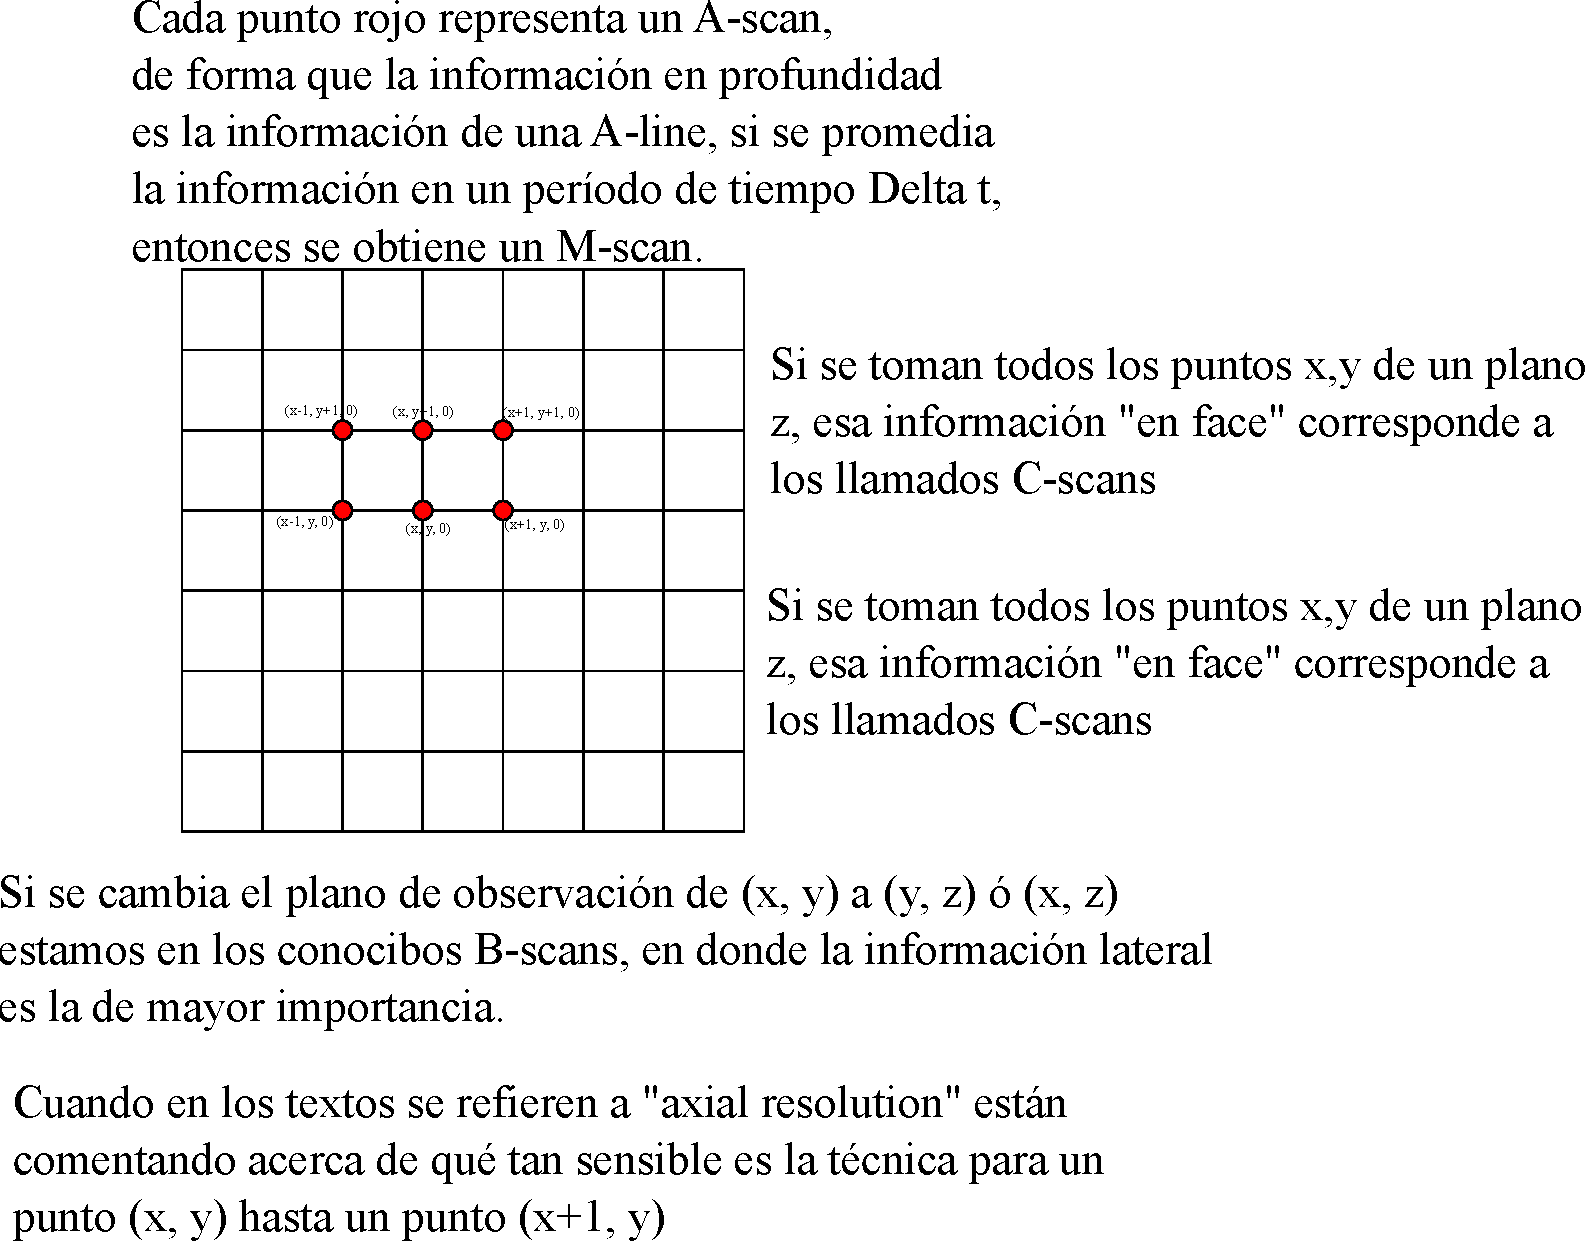
\includegraphics[width=0.7\linewidth]{img/a_scan.pdf}
%	\caption{Interpretación de la resolución axial, y los tipos de escaneos}
%	\label{fig:ascan}
%\end{figure}

%\begin{figure}
%\centering
%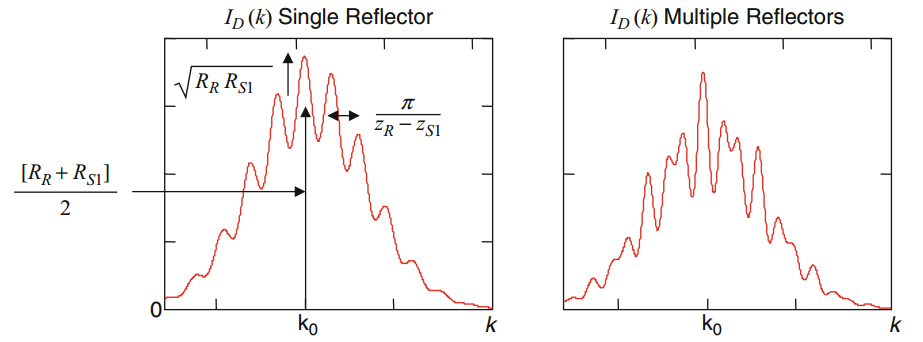
\includegraphics[scale=0.7]{img/gauss_reflect_oct.png}
%\caption{1}
%\label{fig:gaussreflectoct}
%\end{figure}

\subsection{Interferometría de baja coherencia en el dominio del tiempo}

%En la OCT en el dominio del tiempo TDOCT (\textit{time-domain optical coherence tomography}), el barrido no se realiza mediante el cambio del número de onda $k$, sino que a través de diferentes desplazamientos en el espejo de referencia $z_R$ se escanea la reflectividad de la muestra. En este proceso, a diferencia del caso anterior, hay una integración sobre todos los números de onda, de forma que la Eq.~\ref{eq:ID_fin} es convierte en


En la OCT en el dominio del tiempo TDOCT (\textit{time-domain optical coherence tomography}) los escaneos en profundidad se realizan a través del desplazamiento del espejo de referencia, es decir, variaciones en $z_R$. La función encargada de la modulación $\cos[2k(z_R - z_{S_n})]$ aporta información en diferentes frecuencias si se varía la distancia entre el haz referencia y el haz objeto $(z_R - z_{S_n})$, o si bien se modifica el número de onda $k$, siendo ambos procesos equivalentes. Como todo el espectro llega hasta el detector, en la Eq.~\ref{eq:ID_fin} debe realizarse una integración sobre los números de onda, y el patrón de interferencia dependerá entonces de la reflectividad de la muestra y la diferencia de camino óptico. Integrando con respecto a $k$ la Eq.~\ref{eq:ID_fin} se obtiene que

\begin{align}
I_D(z_R) = &\frac{\rho}{4}S_0 [R_R+ R_{S1}+ R_{S2}+...]\\ \notag
&+\frac{\rho}{2}\left[ S_0 \sum_{n=1}^{N} \sqrt{R_R R_{S_n}} e^{-[z_R-z_{S_n}]^2 \Delta k^2}  \cos[2k_0 (z_R-z_{S_n})]\right],
\end{align}

\noindent donde $S_0$ es la potencia de la fuente. En este caso, los términos que aparecen son una componente DC y una función gaussiana que se encuentra modulada por un coseno, cuya frecuencia depende de la longitud de onda central de la fuente $k_0$ y la diferencia de camino entre los brazos. Si se tienen varios reflectores se produce una señal de interferencia en sus posiciones, lo que se ha denominado línea A, esto se ejemplifica en la Fig.~\ref{fig:tdoct}, donde cuatro reflectores muestran interferencia, la señal que se desea medir corresponde justamente a la envolvente de estas funciones. La reflectividad de la muestra se puede encontrar entonces a través de la medida de la modulación que produce la señal portadora (la función coseno) sobre la función gaussiana de cada reflector, además, el ancho de cada función gaussiana está dado por la longitud de coherencia de la fuente.

\begin{figure}[h!]
	\centering
	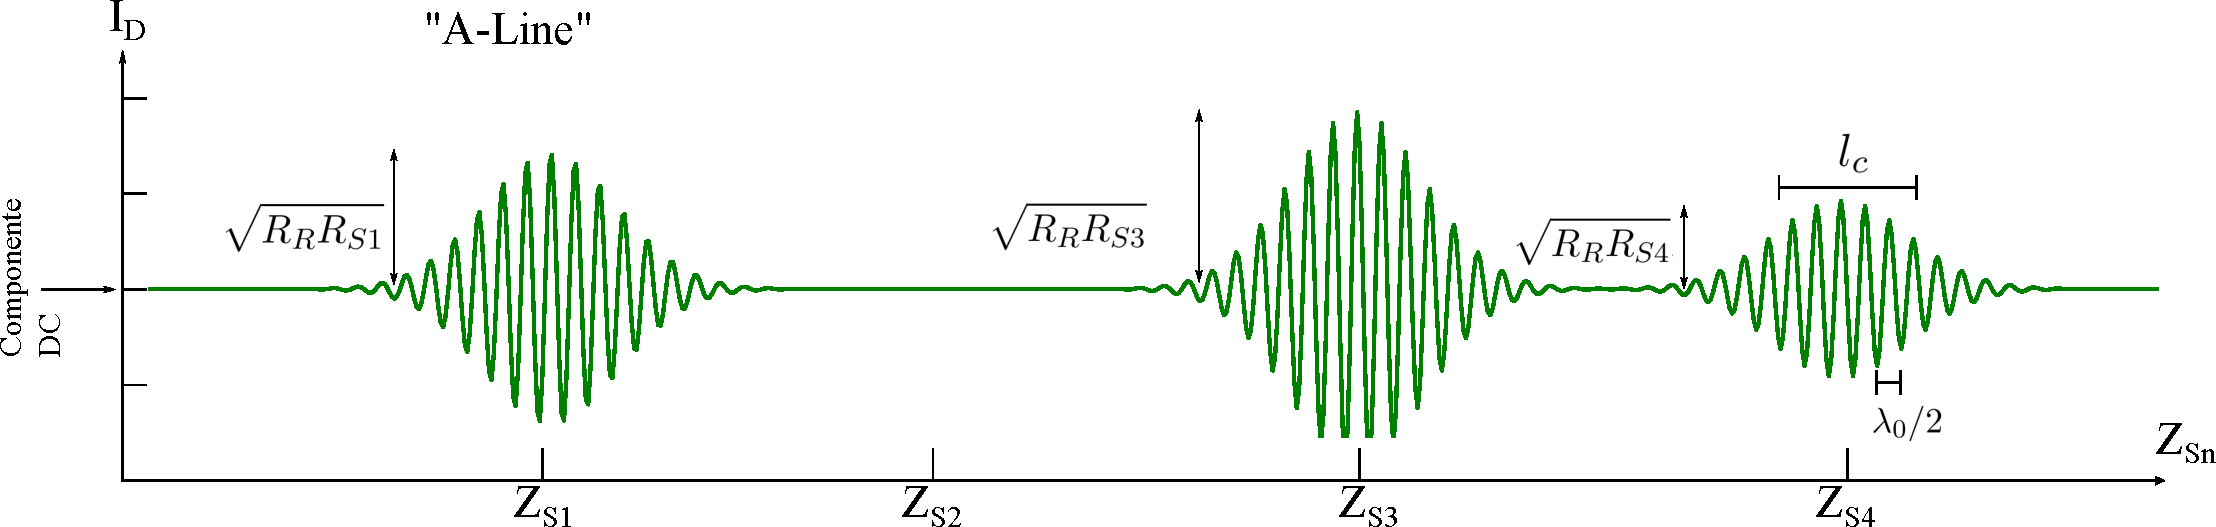
\includegraphics[width=\linewidth,keepaspectratio]{img/A_Line_1Gen}
	\caption{Línea A obtenida cuando se realiza el escaneo a una muestra con cuatro reflectores. La magnitud de la interferencia es lo que se busca medir mediante OCT.}
	\label{fig:tdoct}
\end{figure}


\subsection{Interferometría de baja coherencia en el dominio de Fourier}

En OCT del dominio de Fourier FDOCT (\textit{Fourier-domain optical coherence tomography}), la fotocorriente dependiente del número de onda $I_D(k)$ de la Eq.~\ref{eq:ID_fin} se captura y procesa mediante un análisis de Fourier que permite determinar el perfil de reflectividad $\sqrt{R_S(z_S)}$ de la muestra. En este proceso, el espejo de referencia se mantiene en una posición fija, mientras que las diferentes longitudes de onda son las encargadas de aportar la información de las diferentes profundidades en la muestra. En esta categoría hay dos divisiones para OCT, por un lado se encuentra  la tomografía óptica de coherencia en el dominio espectral SDOCT (\textit{spectral-domain optical coherence tomography}) o tomografía óptica de coherencia basada en espectrómetro. La OCT en el dominio espectral se basa en el empleo de una fuente de luz con banda ancha, con la diferencia de ubicar un espectrómetro en la salida del interferómetro, y todas las componentes frecuenciales de $I_D(k)$ se capturan de manera simultánea. Por otro lado, está la tomografía óptica de coherencia de fuente de barrido SSOCT (\textit{swept-source optical coherence tomography}), llamada también imagen óptica en el dominio frecuencial OFDI (\textit{optical frequency-domain imaging}). En este caso, las componentes espectrales de $I_D(k)$ se obtienen de forma secuencial, capturando la señal de una banda angosta, mientras que la fuente realiza un barrido por las diferentes longitudes de onda.

El perfil de reflectividad de la muestra $r_S(z_S)$ se calcula mediante la transformada inversa de Fourier de la corriente en el fotodetector, tomando en cuenta que la transformada de Fourier de un coseno es $\cos(kz_0) \rightleftarrows 1/2[\delta(z\pm z_0)]$ y la convolución entre funciones se define como el producto de sus transformadas de Fourier $x(z) \otimes y(z) \rightleftarrows X(k)Y(k)$; la transformada inversa de la Eq.~\ref{eq:ID_fin} corresponde a

\begin{align}
\label{eq:i_D_1}
i_D(z) &= \frac{\rho}{8}\left[\gamma (z) [R_R + R_{S1} + R_{S2} + ...] \right]\\ \notag
&+ \frac{\rho}{4} \left[\gamma (z) \otimes \sum_{n=1}^{N} \sqrt{R_R R_{S_n}}\{\delta[z\pm (2(z_R-z_{S_n}))]\}\right]\\
&+ \frac{\rho}{8} \left[\gamma (z) \otimes \sum_{m\neq n = 1}^{N} \sqrt{R_{s_n}R_{s_m}} \{\delta [z\pm 2(z_{S_n} - z_{S_m})]\} \right].\notag
\end{align}

\noindent La convolución de la función $\delta$ con la función coseno se puede calcular mediante sus propiedades, de manera que la Eq.~\ref{eq:i_D_1} corresponde a

\begin{align}
\label{eq:i_D_2}
i_D(z) &= \frac{\rho}{8}\left[\gamma (z) [R_R + R_{S1} + R_{S2} + ...] \right]\\ \notag
&+ \frac{\rho}{4} \left[\sum_{n=1}^{N} \sqrt{R_R R_{S_n}}\{\gamma [2(z_R - z_{S_n}) ] + \gamma[-2(z_R - z_{S_n}) ]\}  \right]\\
&+ \frac{\rho}{8} \left[ \sum_{m\neq n = 1}^{N} \sqrt{R_{S_n}R_{S_m}} \{\gamma [2(z_{S_n} - z_{S_m}) ] + \gamma[-2(z_{S_n} - z_{S_m}) ]\}  \right].\notag
\end{align}

\noindent La Eq.~\ref{eq:i_D_2} es una discretización de la función gaussiana correspondiente a las posiciones de los reflectores de la muestra, lo que se ha denominado línea A (Fig.~\ref{fig:fdoct}).
\begin{figure}[ht!]
	\centering
	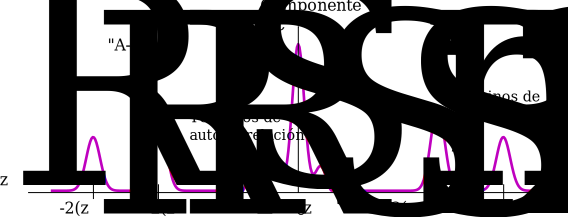
\includegraphics[width=\linewidth]{img/A_Line_FFT}
	\caption{Línea A obtenida en una medición de OCT en el dominio espectral.}
	\label{fig:fdoct}
\end{figure}

La función que se quiere recuperar $\sqrt{R_S(z_S)}$ en este caso se reproduce con las siguientes modificaciones, primero la distancia que se mide desde la posición de referencia está duplicada. El ancho de cada función $\delta$ está dado por la longitud de coherencia de la fuente. En la Eq.~\ref{eq:i_D_1} puede apreciarse claramente la convolución entre la muestra y la distribución de la fuente, esta definición corresponde a la función de dispersión de punto ($PSF$) en un sistema óptico convencional. Finalmente, la aparición de la segunda función $\delta$ se debe al complejo conjugado que resulta de la transformada de Fourier de la función coseno, en general, este término representa ruido en la información que se recupera, sin embargo, existe diferentes técnicas para solucionar este problema \cite{Ho2006,Vergnole2008}.


%\subsection{Interferometría de baja coherencia en el dominio del tiempo}
%
%En el caso de OCT en el dominio del tiempo TDOCT(\textit{time-domain optical coherence tomography}), el barrido no se realiza mediante el cambio del número de onda $k$, sino que a través de diferentes desplazamientos en el espejo de referencia $z_R$ se escanea la reflectividad de la muestra. En este proceso, a diferencia del caso anterior, hay una integración sobre todos los números de onda, de forma que la Eq.~\ref{eq:ID_fin} es convierte en
%
%\begin{align}
%%I_D(k) = &\frac{\rho}{4}S_0 [R_R+ R_{S1}+ R_{S2}+...]\\
%%&+\frac{\rho}{2}\left[ S_0 \sum_{n=1}^{N} \sqrt{R_R R_{S_n}} e^{[-z_R-z_{S_n}]^2 \Delta k^2}  \cos(2k_0 (z_R-Z_{S_n}))\right],
%\end{align}
%
%donde $S_0 = \int_{0}^{\infty} S(k) dk$, que es la energía emitida por la fuente. En este caso, nuevamente los términos que aparecen son una componente DC y una función gaussiana que en este caso se encuentra modulada por el coseno, cuya frecuencia depende de la longitud central de la fuente $k_0$ y la diferencia de camino entre los brazos, esto se ejemplifica en la Fig.~\ref{fig:tdoct}. La reflectividad de la muestra se puede encontrar entonces a través de la medida de la modulación que produce la señal portadora (la función coseno)  sobre la función gaussiana.
%
%\begin{figure}[h!]
%\centering
%-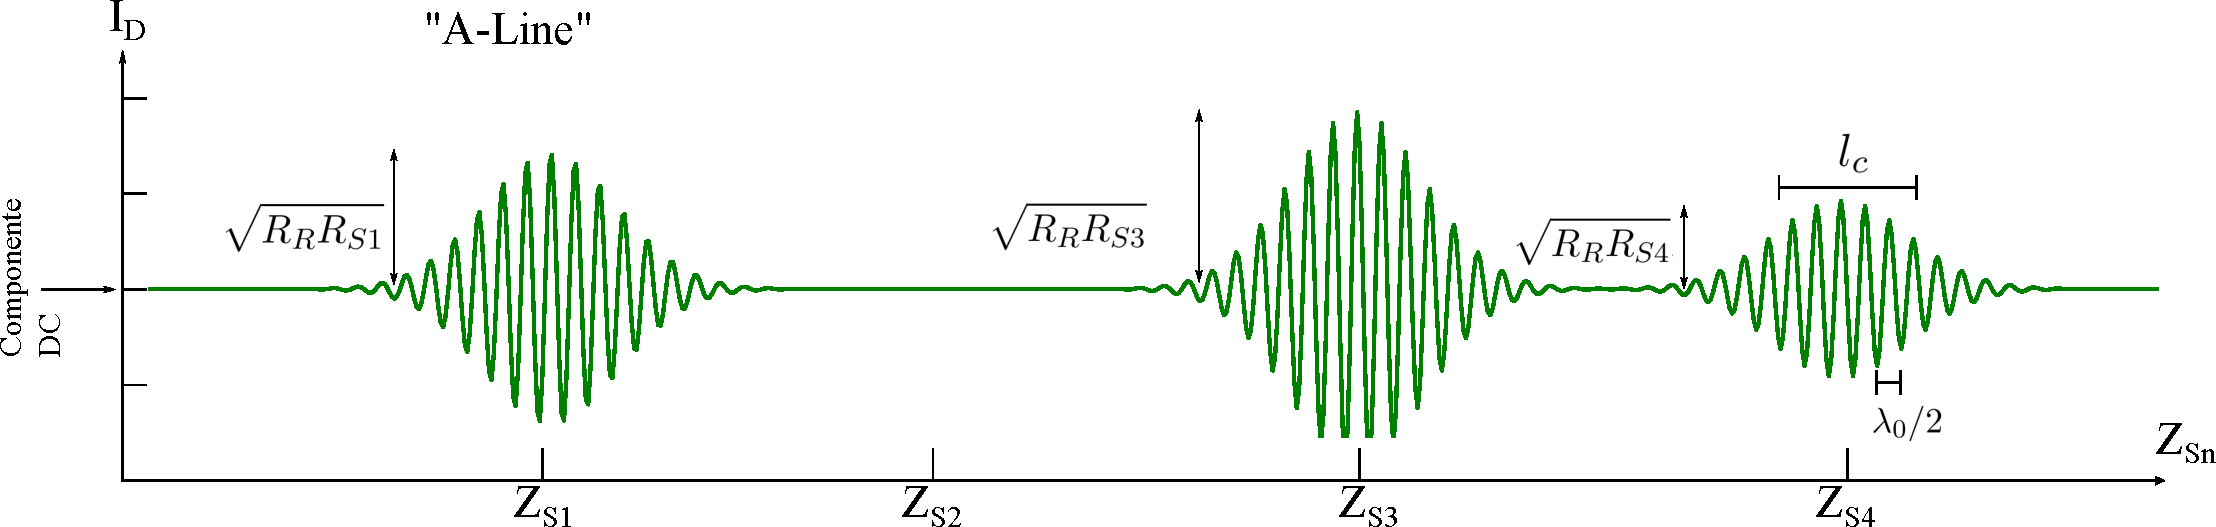
\includegraphics[width=\linewidth,keepaspectratio]{img/A_Line_1Gen}
%\caption{Línea A obtenida cuando se realiza el escaneo a una muestra con cuatro reflectores. La magnitud de la interferencia es lo que se busca medir mediante OCT.}
%\label{fig:tdoct}
%\end{figure}

%\subsection{La relevancia de la OCT en la investigación actual}

%En la actualidad, OCT se ha posicionado como una de las áreas de mayor interés, tanto científico, médico, como comercial. Para ejemplificar esto, en la Fig.~\ref{fig:oct_pub_by_year} se muestra la cantidad de publicaciones relacionadas a OCT desde su aparición hacia 1991. En la figura se aprecia como en los últimos años ha habido un crecimiento exponencial en la cantidad de artículos publicados en el tema, siendo la oftalmología y el estudio cardiovascular las principales áreas de publicación de OCT, datos tomados del US National Library of Medicine National Institutes of Health (http://www.ncbi.nlm.nih.gov/pubmed). Sin embargo, pese su gran expansión, desarrollo y estudio, en latinoamerica son pocos, los grupos de investigación acogen en sus líneas de investigación la OCT, para mostrar esto, en la Fig.~\ref{fig:oct_groups_map_png} se muestra la distribución global de los grupos que publican en OCT. En estos datos sobresalen grupos de universidades como Harvard, la Universidad de California y el MIT, datos tomados del US National Library of Medicine National Institutes of Health (http://www.ncbi.nlm.nih.gov/pubmed). Por último, el mercado de OCT se encuentra en crecimiento, como se indica en la Fig.~\ref{fig:oct_market}, en donde se aprecia que los ingresos de las compañías que producen equipos e indumentaria para OCT para el año 2015 cerró en alrededor de $800$ millones de dólares, lo que muestra un alto potencia para la comercialización e investigación en áreas relacionadas a la OCT, datos tomados del IOVS: Investigative Ophthalmology \& Visual Science.
%
%\begin{figure}[ht!]
%\centering
%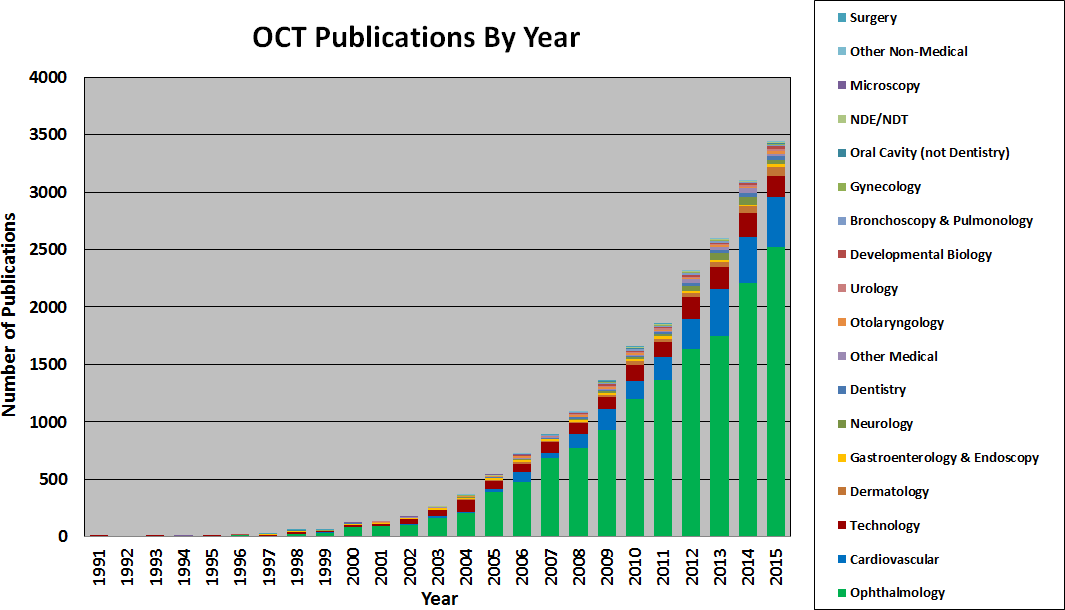
\includegraphics[width = \textwidth, keepaspectratio]{img/oct_pub_by_year.png}
%\caption[Citaciones sobre OCT en los últimos años.]{Citaciones sobre OCT en los últimos años. Tomado de http://www.ncbi.nlm.nih.gov/pubmed .}
%\label{fig:oct_pub_by_year}
%\end{figure}

%\begin{figure}[ht!]
%\centering
%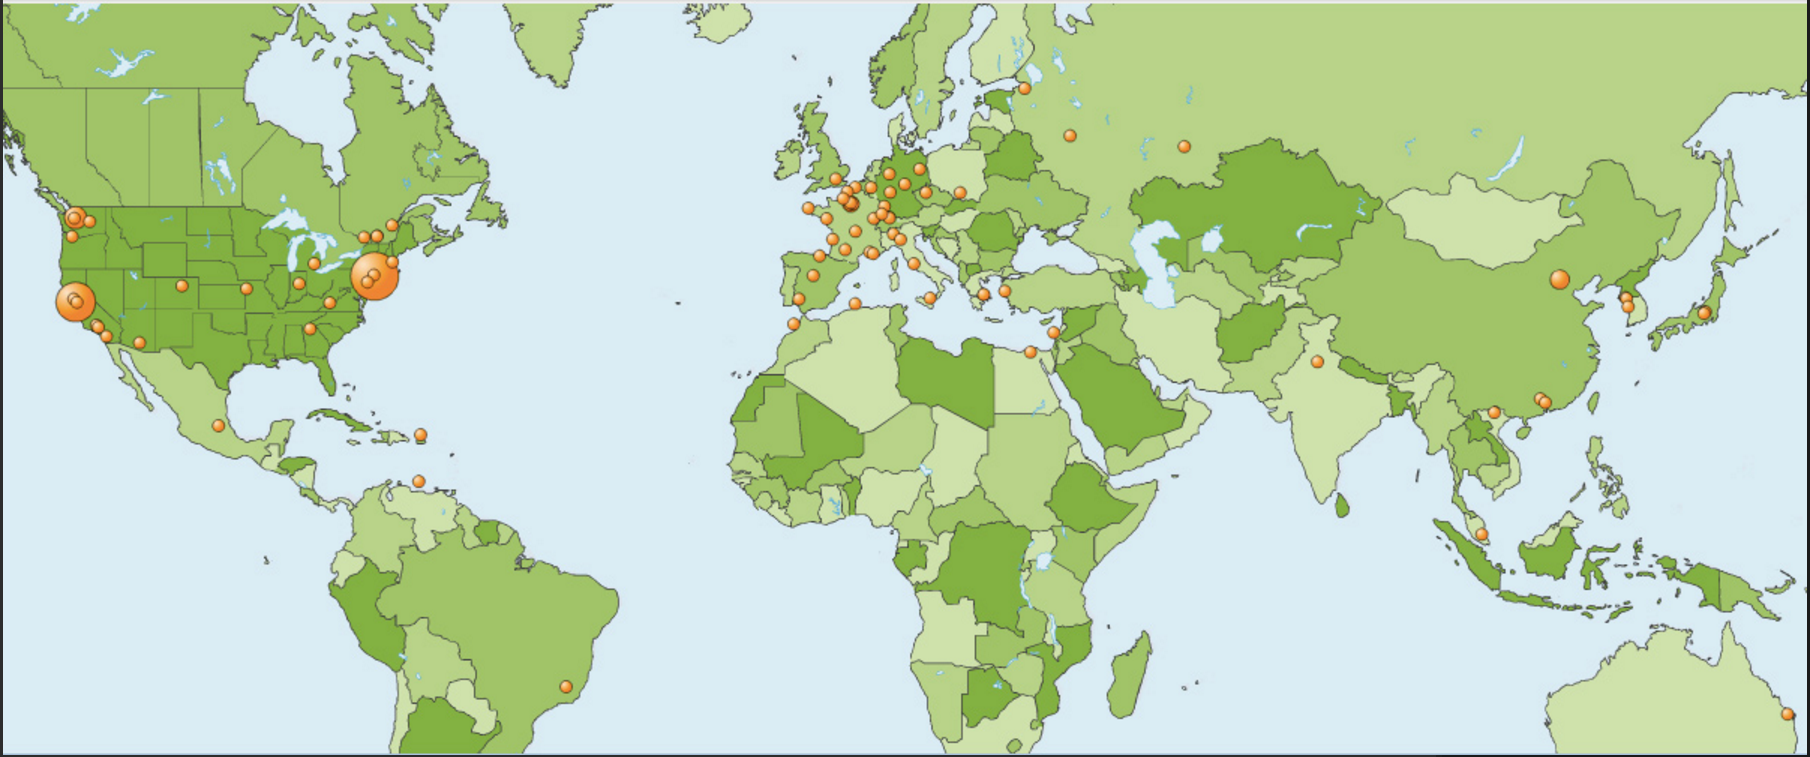
\includegraphics[width = \textwidth, keepaspectratio]{img/oct_groups_map_png.png}
%\caption[Mapa global de los grupos que investigan en OCT.]{Mapa global de los grupos que investigan en OCT. Tomada del Insihgt: OCT market http://www.sweptlaser.com/OCT-market .}
%\label{fig:oct_groups_map_png}
%\end{figure}

%\begin{figure}[ht!]
%\centering
%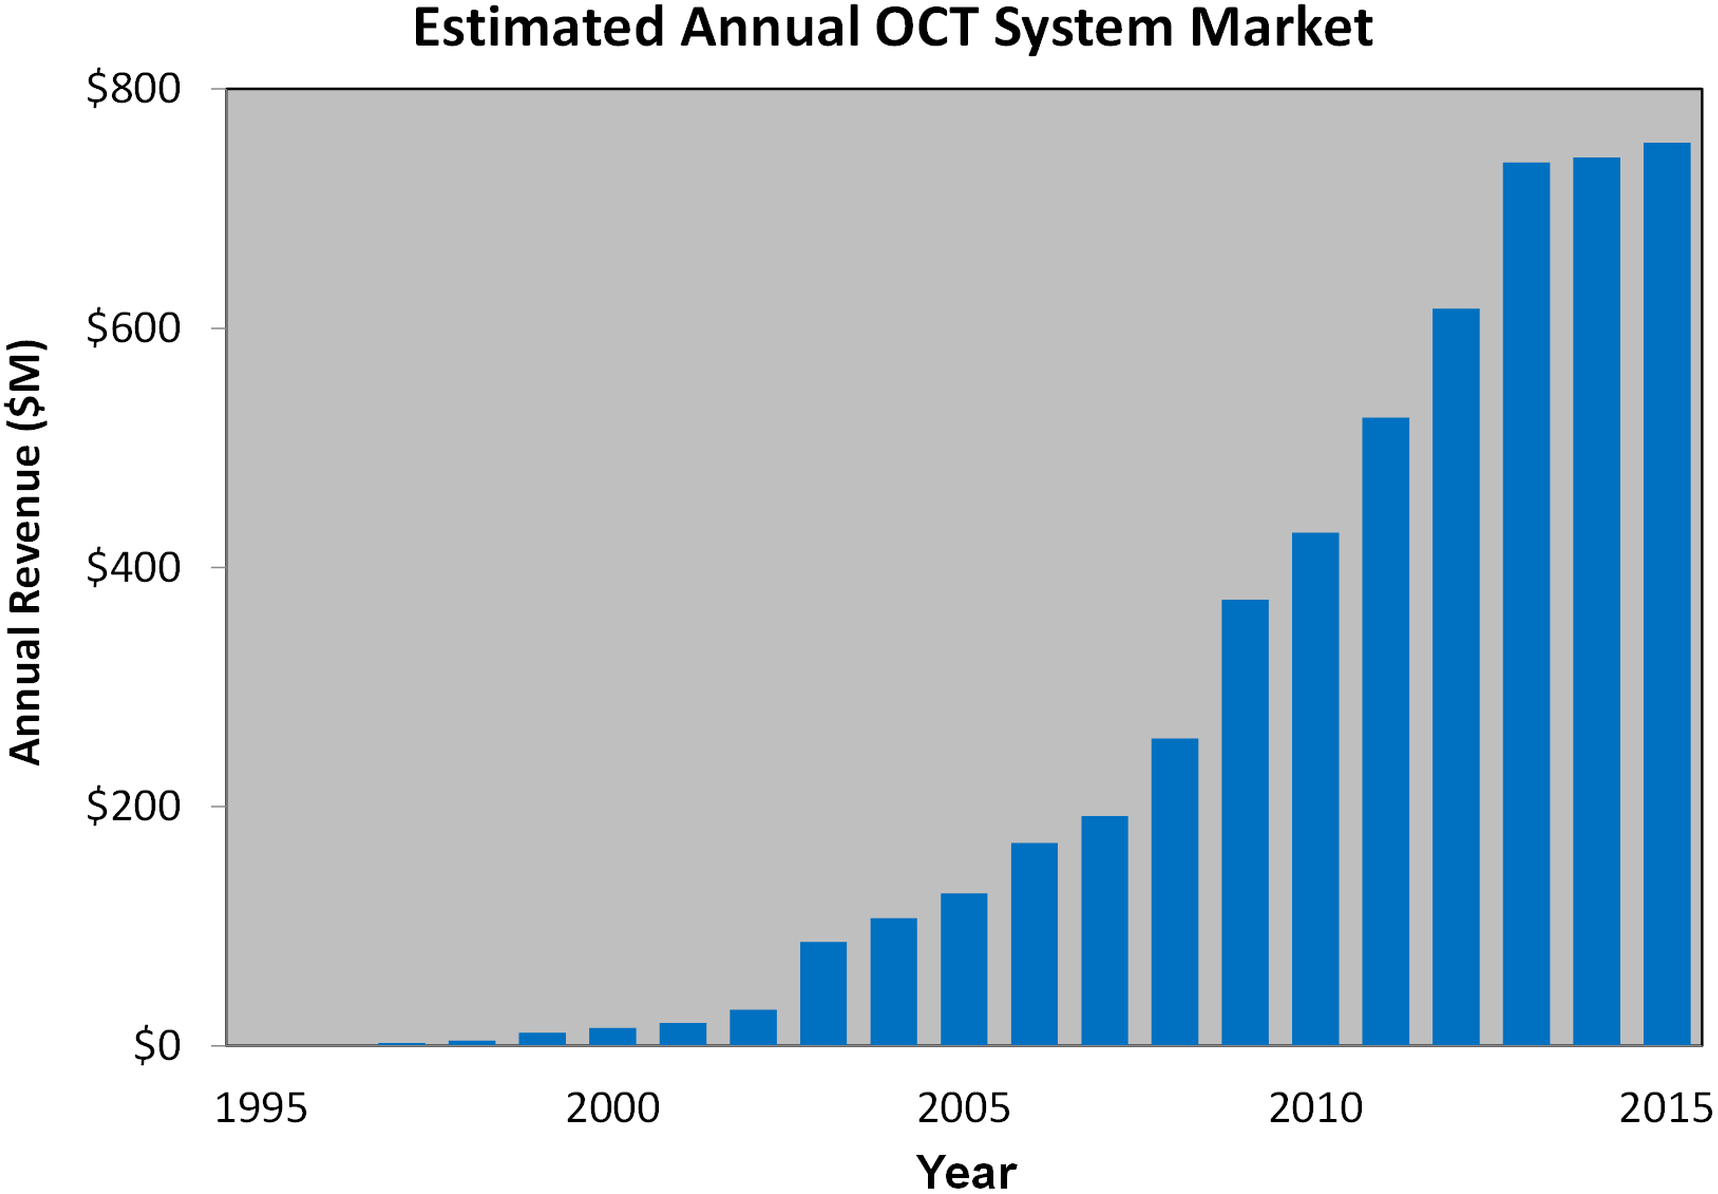
\includegraphics[width = \textwidth, keepaspectratio]{img/oct_market}
%\caption[Mercado de OCT.]{Mercado de la OCT en los últimos años, datos tomados de: http://iovs.arvojournals.org/.}
%\label{fig:oct_market}
%\end{figure}

%\subsection{Objetivos}
%\subsubsection{Objetivo general}
%
%%Desarrollar métodos de optimización en paralelo para la identificación de objetos de fase para la tomografía óptica coherente para diagnosis médico.
%%Mejorar la identificación de objetos de fase en tomografía óptica coherente mediante optimización en paralelo, que ayuden en el diagnosis médico.
%Estabilizar mediante posprocesamiento la fase en tomografía óptica de coherencia.
%
%\subsubsection{Objetivos específicos}
%
%\begin{itemize}
%	\item Identificar el estado de arte de la tomografía óptica coherente en aplicaciones biomédicas.
%%	\item Implementar un sistema óptico equivalente a los montajes utilizados durante la primera generación de la tomografía óptica coherente.
%	\item Implementar un sistema óptico de prueba de concepto de campo completo en la tomografía de coherencia óptica.
%%	\item Simular un volumen de datos que represente un objeto característico encontrados en la tomografía óptica coherente.
%%	\item Simular un volumen de datos que posea las características de los objetos que se pueden encontrar en la tomografía óptica coherente, incluyendo las corrupciones de fase provenientes del muestreo.
%	\item Realizar una simulación del muestreo y la formación de imagen en tomografía óptica de coherencia, incluyendo elementos de corrupción de fase.
%%	\item Desarrollar y aplicar un método de optimización de fase que permita encontrar las características del objeto simulado anteriormente.
%	\item Desarrollar un método de optimización de fase que permita recuperar el mapa de corrupción de la imagen simulada anteriormente.
%%	\item Definir una métrica del error para evaluar la convergencia del algoritmo de optimización propuesto.
%	\item Comprobar experimentalmente la funcionalidad del algoritmo propuesto con datos experimentales suministrados por el \emph{Wellman Center for Photomedicine, Harvard Medical School and Massachusetts General Hospital}.
%\end{itemize}


%\section{Conclusión}


	\section{Objetivos}
\label{sec:objetivos}
\subsection{Objetivo General}
%Desarrollar métodos de optimización en paralelo para la identificación de objetos de fase para la tomografía óptica coherente para diagnosis médico.
%Mejorar la identificación de objetos de fase en tomografía óptica coherente mediante optimización en paralelo, que ayuden en el diagnosis médico.
Estabilizar la fase en tomografía óptica de coherencia mediante posprocesamiento.

\subsection{Objetivos Específicos}

\begin{itemize}
	\item Identificar el estado de arte de la tomografía óptica de coherente en aplicaciones biomédicas.
	%	\item Implementar un sistema óptico equivalente a los montajes utilizados durante la primera generación de la tomografía óptica coherente.
	\item Implementar un sistema óptico de prueba de concepto de campo completo en la tomografía de coherencia óptica.
	%	\item Simular un volumen de datos que represente un objeto característico encontrados en la tomografía óptica coherente.
	%	\item Simular un volumen de datos que posea las características de los objetos que se pueden encontrar en la tomografía óptica coherente, incluyendo las corrupciones de fase provenientes del muestreo.
	\item Realizar una simulación del muestreo y la formación de imagen en la tomografía óptica de coherencia, incluyendo elementos de corrupción de fase.
	%	\item Desarrollar y aplicar un método de optimización de fase que permita encontrar las características del objeto simulado anteriormente.
	\item Desarrollar un método de posprocesamiento que permita recuperar el mapa de corrupción de la imagen simulada anteriormente.
	%	\item Definir una métrica del error para evaluar la convergencia del algoritmo de optimización propuesto.
	\item Comprobar experimentalmente la funcionalidad del algoritmo propuesto con datos experimentales suministrados por el \emph{Wellman Center for Photomedicine, Harvard Medical School and Massachusetts General Hospital}.
	
\end{itemize}


\section{Metodología}
\label{sec:metodologia}

Para el desarrollo del trabajo de grado se proponen cinco etapas metodológicas. La primera etapa consiste en la búsqueda bibliográfica y revisión de conceptos fundamentales para el desarrollo del trabajo de grado. La segunda etapa es el estudio teórico y la simulación que permitan implementar los conceptos adquiridos y así generar datos con características conocidas. La tercera etapa consiste en el desarrollo e implementación de algoritmos o procedimientos que permitan resolver el problema planteado anteriormente. La cuarta etapa comprende la puesta práctica de los algoritmos y técnicas desarrollados con datos obtenidos de pacientes en sistemas reales. La última etapa consiste en la validación de los resultados mediante la publicación y la documentación del trabajo de grado.

\subsection{Revisión bibliográfica}

%La revisión bibliográfica es una etapa fundamental en el desarrollo de cualquier actividad investigativa, ya que a partir de las bases teóricas es posible entender los conceptos que fundamentan las propuestas actuales reportadas en la literatura, esta etapa permite también identificar aquellas áreas en las cuales puede mejorarse o modificarse las propuestas actuales e incluso plantear nuevas. La revisión bibliográfica aunque se realizará a lo largo del desarrollo del trabajo de grado, tendrá una mayor importancia al inicio de las actividades. Para el comienzo del trabajo de grado esta actividad se encuentra desarrollada en un $70\%$, los conceptos básicos ya se asumen como apropiados y el restante de la revisión bibliográfica corresponde a una actividad complementaria a la documentación y generación de resultados.

La revisión bibliográfica es una etapa fundamental en el desarrollo de cualquier actividad investigativa, ya que a partir de las bases teóricas es posible entender los conceptos que fundamentan las propuestas actuales reportadas en la literatura y permite brindar un fundamento teórico que explique cómo las propuestas que se realicen pueden efectivamente aportar una solución al problema planteado. La revisión bibliográfica aunque se realizará a lo largo del desarrollo del trabajo de grado, tendrá una mayor importancia al inicio de las actividades. Para el comienzo del trabajo de grado esta actividad se encuentra desarrollada en un $70\%$, los conceptos básicos ya se asumen como apropiados y el restante de la revisión bibliográfica corresponde a una actividad complementaria a la documentación y generación de resultados.

\subsection{Estudio teórico y simulación}

Con una base teórica y conociendo los desarrollos actuales en el área, es posible plantear desde un punto de vista teórico cuáles de las propuestas realizadas como mejoras, modificaciones o implementaciones puede representar la solución más óptima al problema. En esta etapa se busca definir los conceptos de las propuestas, para así identificar una ruta sobre la cuál desarrollar las actividades del trabajo de grado. 

La simulación es una forma de probar las técnicas propuestas a partir de datos que permiten identificar la veracidad y viabilidad experimental que tendrían las propuestas realizadas. La simulación comprende desde el uso de la teoría en la generación de datos con características conocidas, hasta la aplicación experimental de las propuestas conociendo los resultados que se deben obtener. En el desarrollo del trabajo de grado, esta etapa comienza con un avance del $50\%$, siendo ese primer desarrollo, la aplicación inicial de los conceptos para la simulación y recuperación de datos inicial. El porcentaje faltante se encuentra en la aplicación de elementos de corrupción que sean identificables.

\subsection{Desarrollo e implementación}

En esta etapa se realizarán los desarrollos teóricos y computacionales requeridos para la implementación de algoritmos que basados en las propuestas realizadas, solucionan el problema de este trabajo de grado. La aplicación computacional inicialmente con los datos simulados permite identificar las deficiencias y componentes que podrían ser mejoradas en los algoritmos propuestos. Entre las mejoras más comunes que se pueden incorporar se encuentran: reducción en el tiempo de procesamiento, menor sensibilidad ante el ruido, independencia de los datos iniciales, entre otros.

Para el trabajo de grado, esta etapa comienza en un $40\%$ de desarrollo, correspondiente a aplicaciones iniciales de algoritmos de prueba, el porcentaje restante está relacionado con la adaptación de más elementos que permitan al algoritmo tener un funcionamiento óptimo en diferentes tipos de datos.

\subsection{Aplicación experimental}

Luego de que se tenga un algoritmo que funcione con los datos simulados, se procedería a realizar la validación experimental con datos provenientes de pacientes. Con esta implementación se espera que de los datos obtenidos inicialmente sea posible obtener más información sin la necesidad de ingresar nuevamente en el paciente. Como se planteó en el problema, el objetivo es poder identificar el mapa de corrupción de la fase y así obtener la fase real del tomograma. 

Debido a que la toma de datos en pacientes se encuentra regulada por normas internacionales, los datos experimentales los proveerá el \emph{Wellman Center for Photomedicine}, quienes cuentan con la instrumentación requerida y cumplen los requisitos de seguridad para obtener imágenes al interior de los pacientes. En esta actividad aun no hay ningún avance, ya que los algoritmos no se encuentran terminados.

\subsection{Publicación y documentación de resultados}

Uno de los productos de investigación más importante para las instituciones de educación sin lugar a duda son las publicaciones. En este sentido, se espera que del desarrollo del trabajo de grado se obtenga al menos una publicación internacional que dé cuenta de la validez científica a las propuestas, implementaciones y resultados obtenidos. Asimismo, se espera la participación en congresos especializados sobre el tema, que permitan la interacción y difusión de los resultados del trabajo de grado. Esta etapa comprende también la escritura de la tesis como documento final que recopila toda la información que ha sido empleada a lo largo del trabajo de grado. 
	\section{Cronograma}
\label{sec:cronograma}

El cronograma con los tiempo de desarrollo para cada una de las actividades se presenta en la Fig.~\ref{fig:cronogramalisto}. Para la ejecución del trabajo de grado se proponen cuatro etapas divididas en: evaluación del problema, simulación, desarrollo y experimentación. A continuación se detalla el proceso y los productos esperados en cada una de las actividades:


1. \textit{Identificar el estado de arte de la tomografía óptica coherente en aplicaciones biomédicas}. En este paso se busca crear un fundamento teórico y entendimiento del problema que se abordará en el trabajo de grado, lo cual se realizará mediante la lectura de artículos en revistas especializadas, tales como: \emph{Optics letters}\footnote{\url{https://www.osapublishing.org/ol/home.cfm}}, \emph{Biomedical optics express}\footnote{\url{https://www.osapublishing.org/boe/home.cfm}}, \emph{Journal of biomedical optics}\footnote{\url{https://spie.org/publications/journals/journal-of-biomedical-optics}}, \emph{Science}\footnote{\url{http://www.sciencemag.org/}}, entre otras del área óptica y biomédica. Con este proceso se entenderán conceptos fundamentales acerca del principio físico, funcionamiento y evolución de la tomografía óptica de coherencia. Esta faceta incluye la revisión constante de literatura para comprender y explicar los problemas que puedan surgir en etapas futuras.

2. \textit{Escribir anteproyecto del trabajo de grado}. Esta actividad busca obtener un documento resumen en el cual se plantea de manera clara el problema que se abordará para el trabajo de grado, en este busca depositarse el marco teórico y los conceptos básicos necesarios para el desarrollo del trabajo.


\begin{figure}[H]
	\centering
	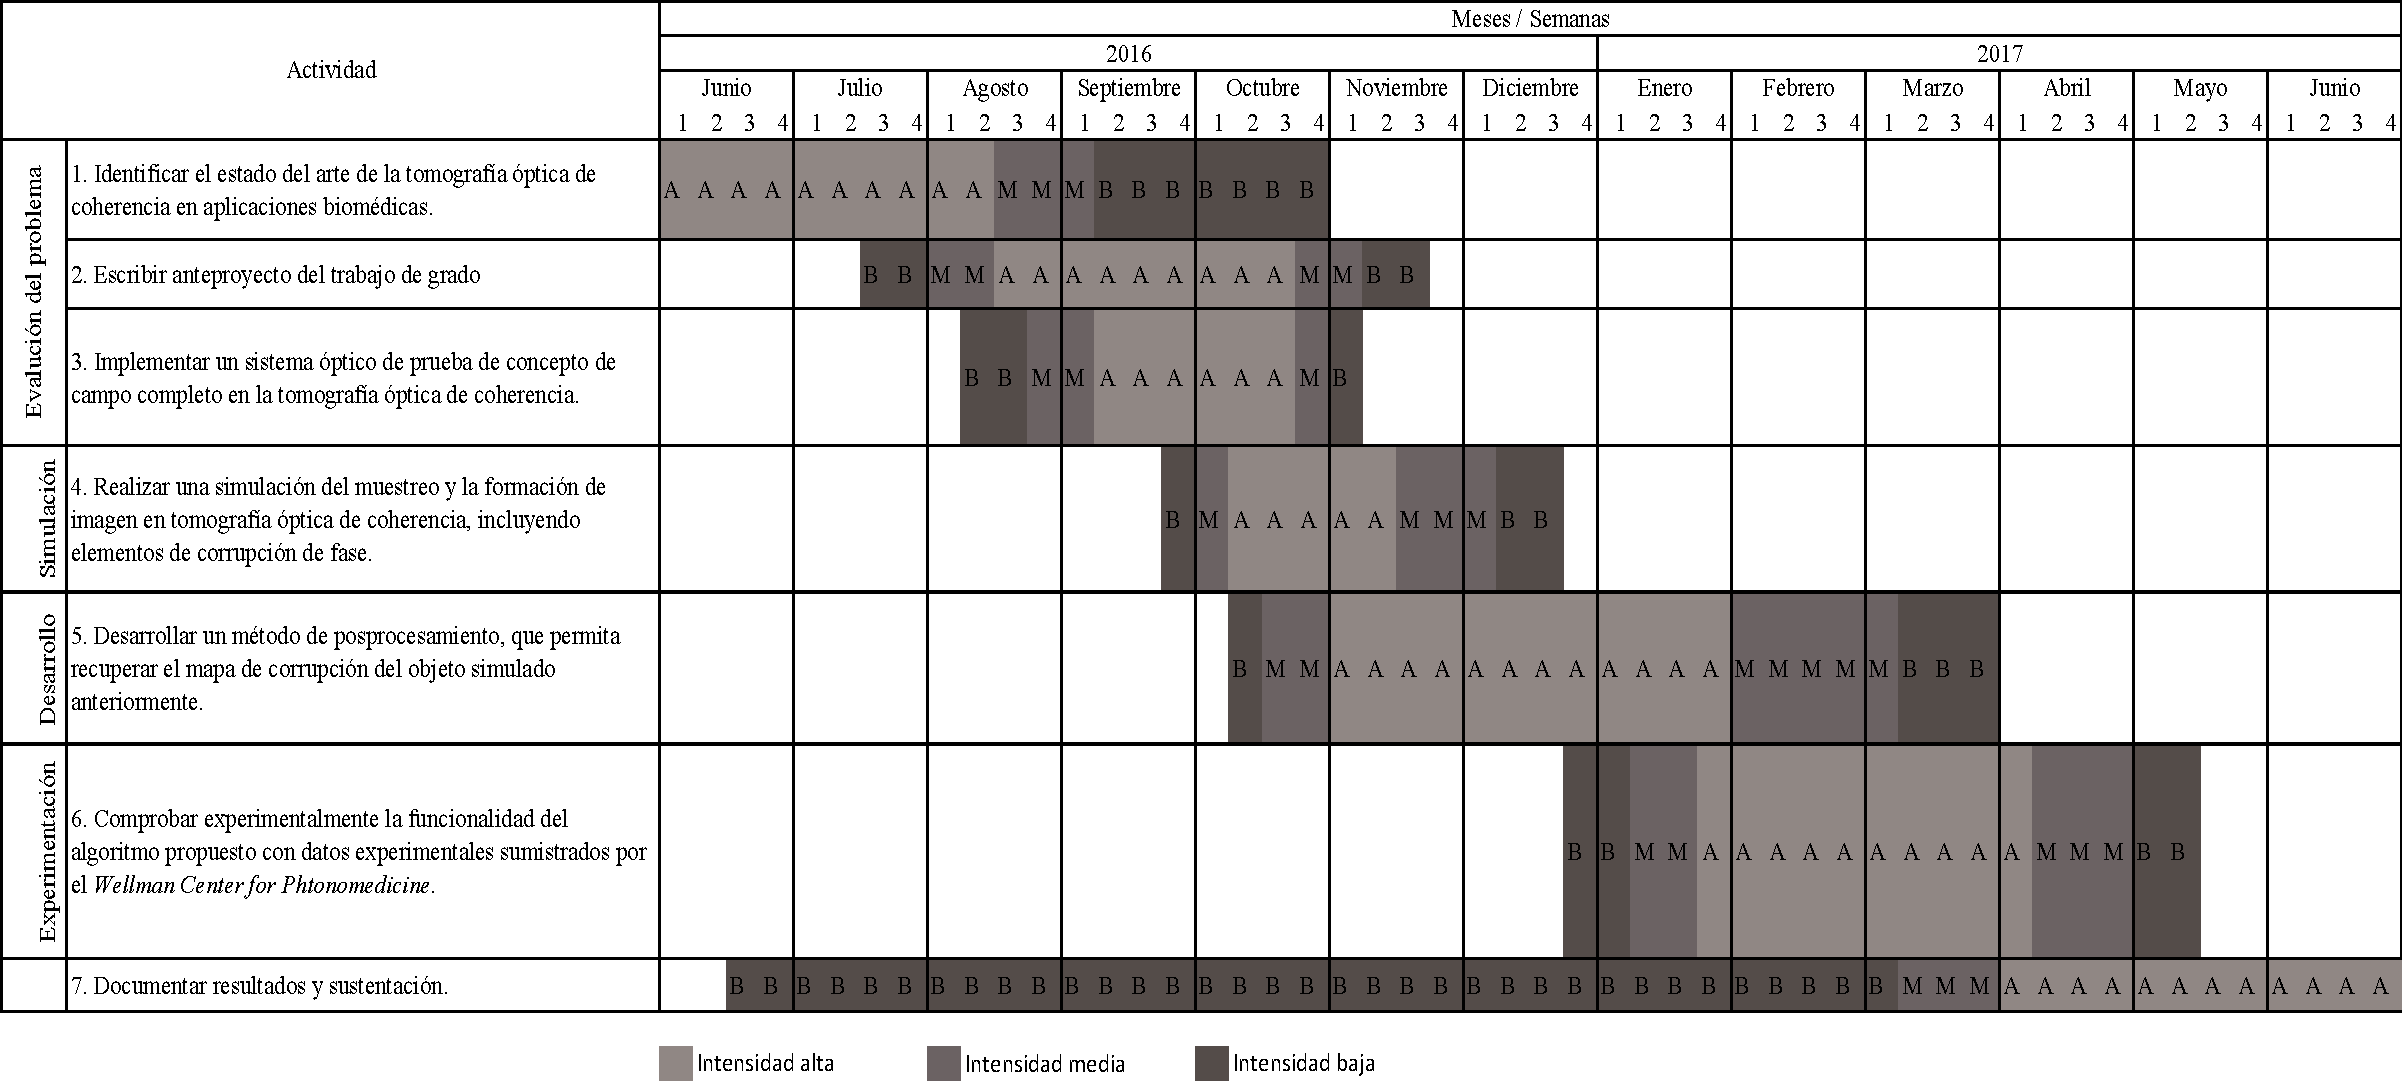
\includegraphics[scale=0.5, angle = 90]{Cronograma_listo.pdf}
	\caption[Cronograma de actividades.]{Cronograma de actividades.}
	\label{fig:cronogramalisto}
\end{figure}


3. \textit{Implementar un sistema óptico de prueba de concepto de campo completo en la tomografía de coherencia óptica}. Se implementará un interfómetro de Michelson con luz blanca, en donde el haz de referencia pueda ser desplazado con respecto al haz objeto, de esta manera se tendrá un sistema de OCT de primera generación con el cual se entenderán fenómenos y problemas que allí se presentan. A este sistema de OCT se le llama de campo completo debido a que la reflectividad de la luz en función de la profundidad es medida directamente para un plano usando una cámara CCD. En este montaje se planea utilizar dos objetos diferentes: el primer objeto que se empleará es un elemento traslucido con dos superficies, de forma que mediante el sistema de OCT se recuperará la separación entre las caras del objeto mediante la medición de la retroreflexión producida por el cambio del índice de refracción del medio. La segunda etapa consistirá en emplear un material traslucido y dispersivo, cuyas características se asemejen  a las muestras empleadas en OCT, de forma que mediante la retrodispersión producida por la muestra se obtendrá el mapa de reflectividad en función de la profundidad. 


4. \textit{Realizar una simulación del muestreo y la formación de imagen en tomografía óptica de coherencia, incluyendo elementos de corrupción de fase}. Esta etapa busca simular la formación de imagen en los sistemas de tomografía óptica de coherencia, mediante esta simulación se busca obtener un volumen de datos sobre los cuales se realizarán las primeras pruebas con los algoritmos desarrollados. En principio, se obtendrán datos para objetos conocidos empleando conceptos de OCT, luego computacionalmente se agregarán las características que poseen las imágenes obtenidas experimentalmente, esto incluye corrupciones en la fase por desalineamientos indeseados en la adquisición de las imágenes, así como la presencia de moteado por la dispersión de la luz. El objetivo final será poder reproducir mediante los algoritmos propuestos los mapas de corrupción que fueron añadidos en las imágenes.

5. \textit{Desarrollar un método de posprocesamiento que permita recuperar el mapa de corrupción de la imagen simulada anteriormente}. Con los datos simulados en el objetivo anterior, se desarrollará un algoritmo que permita encontrar los elementos de corrupción en la fase para el volumen de datos. La propuesta inicial consiste en emplear algoritmos de enfoque para medios turbios, en los cuales mediante posprocesamiento recuperan la fase que produce el mejor enfoque del haz cuando este se propaga en un medio turbio. De manera similar este concepto podría emplearse en OCT si se considera que cuando el haz de entrada posee un perfil gaussiano y adicionalmente la fase no está corrupta, el enfoque de este haz debe producir otro haz gaussiano, situación que no sucede cuando la fase está corrupta. Adicionalmente, consiste en la implementación de algoritmos que permitan la reducción de moteado, de forma que la fase pueda ser reconstruida de una manera más sencilla.

6. \textit{Comprobar experimentalmente la funcionalidad del algoritmo propuesto con datos experimentales suministrados por el \emph{Wellman Center for Photomedicine, Harvard Medical School and Massachusetts General Hospital}}. Los resultados obtenidos de las simulaciones se emplearán para corregir imágenes que provienen de datos experimentales de OCT, ya que en el laboratorio no se cuenta con un sistema de OCT de segunda generación que cumpla con las características requeridas para ser usado en pacientes, los datos serán suministrados por el co-asesor de este trabajo de grado. Con esto se espera validar los resultados obtenidos de manera experimental.

7. \textit{Documentación de resultados}. Los resultados serán de este trabajo de grado serán entregados a modo de documento, acompañado por la sustentación del mismo.

\section{Recursos}
\label{sec:recursos}

El desarrollo del trabajo de grado se realizará principalmente en el Laboratorio de Fotónica de la Universidad EAFIT que cuenta con los recursos e instrumentos necesarios para la realización de cada casi todas las actividades. Las implementaciones computacionales requieren de un equipo de computo con acceso a herramientas de programación tales como MATLAB, C++, Python y LabView;  de un sistema de computación en paralelo con arquitectura GPU y de los periféricos básicos, este sistema lo posee el Laboratorio de Fotónica. Para la realización del montaje de prueba, los instrumentos tales como la mesa óptica, espejos, divisores de haz, fuente de luz, piezoeléctricos y cámaras también se encuentran en las instalaciones del Laboratorio. El sistema de OCT que cumple con los requisitos de seguridad para la toma de muestras en pacientes, así como los componentes necesarios para la adquisición de datos y la toma de algunos datos, será realizada por el \emph{Wellman Center for Photomedicine}.

El recurso humano será aportado por las dos instituciones involucradas en este trabajo de grado, desde la Universidad EAFIT con el profesor e investigador René Restrepo quien será el asesor principal, desde el \emph{Wellman Center for Photomedicine} el Ph.D. Néstor Uribe-Patarroyo, se encargará también del asesoramiento en el desarrollo del trabajo de grado en calidad de co-asesor.

	\addcontentsline{toc}{section}{Referencias}
	\bibliography{bib/Referencias}
	\bibliographystyle{unsrt}
	
\end{document}